\documentclass[sigplan,screen]{acmart}
\let\Bbbk\relax
\usepackage[english, provide=*]{babel}
\usepackage[T1]{fontenc}
\usepackage{amsmath, amsfonts, amssymb}
\usepackage{graphicx}
\usepackage{mathpartir}
\usepackage{pmboxdraw}
\usepackage{hyperref}
\usepackage{listings}
\usepackage{etoolbox}
\apptocmd{\thebibliography}{\raggedright}{}{}
\usepackage{xr}
\externaldocument[supp-]{supplementary}
\usepackage{geometry}
\geometry{margin=1in}
\usepackage{tikz}
\usetikzlibrary{shapes.geometric, shapes.multipart, arrows.meta, positioning, calc}

\tikzstyle{startstop} = [rectangle, rounded corners, minimum width=3cm, minimum height=1cm,text centered, draw=black, fill=gray!20]
\tikzstyle{process} = [rectangle, minimum width=3cm, minimum height=1cm, text centered, draw=black, fill=blue!10]
\tikzstyle{decision} = [diamond, aspect=2, draw=black, fill=orange!20, text centered]
\tikzstyle{arrow} = [thick, ->, >=stealth]

\raggedbottom
\overfullrule = 1cm

% Manually define \xRightarrow since it's not working
\newcommand{\xRightarrow}[1]{\overset{#1}{\Rightarrow}}

% Manually define JSON listing format
\lstdefinelanguage{json}{
	basicstyle=\normalfont\ttfamily,
	numbers=left,
	numberstyle=\scriptsize,
	stepnumber=1,
	numbersep=8pt,
	showstringspaces=false,
	breaklines=true,
	frame=lines
}

\title{TreeLock: Merkle Tree-Based Inheritance in Decentralized Module Systems}

\author{S. C. Dunn}
\affiliation{%
\institution{Starlabs, LLC}
\city{Colorado Springs}
\state{CO}
\country{USA}}
\email{starlabsactual@gmail.com}
\date{\today}

\begin{CCSXML}
	<ccs2012>
		<concept>
			<concept_id>10011007.10011006.10011041</concept_id>
			<concept_desc>Software and its engineering~Compilers</concept_desc>
			<concept_significance>300</concept_significance>
		</concept>
		<concept>
			<concept_id>10011007.10011006.10011060.10011061</concept_id>
			<concept_desc>Software and its engineering~Software configuration management and version control systems</concept_desc>
			<concept_significance>500</concept_significance>
		</concept>
		<concept>
			<concept_id>10011007.10010940.10010971</concept_id>
			<concept_desc>Software and its engineering~Distributed programming languages</concept_desc>
			<concept_significance>300</concept_significance>
		</concept>
		<concept>
			<concept_id>10003752.10010124.10010138</concept_id>
			<concept_desc>Theory of computation~Program semantics</concept_desc>
			<concept_significance>300</concept_significance>
		</concept>
		<concept>
			<concept_id>10003752.10010124.10010131.10010133</concept_id>
			<concept_desc>Theory of computation~Type structures</concept_desc>
			<concept_significance>300</concept_significance>
		</concept>
		<concept>
			<concept_id>10002978.10003029.10003032</concept_id>
			<concept_desc>Security and privacy~Cryptographic protocols</concept_desc>
			<concept_significance>300</concept_significance>
		</concept>
	</ccs2012>
\end{CCSXML}

\ccsdesc[500]{Software and its engineering~Software configuration management and version control systems}
\ccsdesc[300]{Software and its engineering~Compilers}
\ccsdesc[300]{Software and its engineering~Distributed programming languages}
\ccsdesc[300]{Theory of computation~Program semantics}
\ccsdesc[300]{Theory of computation~Type structures}
\ccsdesc[300]{Security and privacy~Cryptographic protocols}

\keywords{content-addressed modules, Merkle trees, decentralized registries, module resolution, module inheritance, type safety, generics, structural typing, inheritance, semantic versioning, reproducibility, distributed systems}

\begin{document}

\begin{abstract}
Modern software module systems face challenges in securely and efficiently resolving dependencies across decentralized and evolving codebases. This paper introduces a novel Merkle tree-based inheritance and resolution model that enables secure, deterministic, and incremental module finalization by capturing complete ancestry traces in a cryptographically verifiable manner. My approach formalizes symbol resolution and override semantics over inheritance DAGs, allowing for conflict detection and transparent override traceability. I present a scalable resolution algorithm and demonstrate its theoretical scalability through synthetic benchmarks simulating diverse module graph topologies. To validate feasibility, I outline a prototype implementation leveraging decentralized lookup protocols and WebAssembly-based evaluation. This model supports improved cacheability, fault tolerance, and tooling integration, positioning it as a promising foundation for future secure and decentralized module management systems.
\vfill
\end{abstract}

\maketitle

\section{Introduction}

Modern software development depends on large collections of independently authored modules. These modules evolve separately, follow distinct versioning patterns, and often depend on one another through complex relationships. Despite this complexity, developers expect module systems to provide predictable behavior, safe composition, and reproducible builds.

In this paper, I introduce a new approach to module resolution that treats each module as a symbolic commitment to its entire ancestry and override history. Instead of resolving names dynamically or relying on external registries to determine behavior, the system finalizes modules into cryptographic Merkle roots that represent their complete inheritance trace. These roots capture not only the content of the module but also the structure of its dependencies, the override relationships between symbols, and the path taken to produce each result.

This approach reframes module resolution as a form of symbolic hashing. The system walks an acyclic inheritance graph, tracks override sites, and computes a canonical resolution trace. The result is both deterministic and portable. Finalized modules can be distributed, cached, or compared without requiring access to their source trees. Symbol lookups are fast and reproducible, and resolution failures can be traced and understood in symbolic form.

The prototype implementation, called \texttt{Tangl}, demonstrates these ideas in practice \cite{tangl}. It supports decentralized resolution using content-addressed inheritance and produces deterministic override traces. Although early in development, the tool is capable of resolving complex module graphs and is designed to integrate with existing development workflows such as continuous integration and version control.

The main contributions of this work are:

\begin{itemize}
	\item A symbolic module model based on immutable inheritance graphs
	\item A deterministic resolution algorithm that produces Merkle roots and override traces
	\item A reference implementation that supports decentralized caching and symbolic analysis
	\item An evaluation using synthetic module topologies to demonstrate scalability and reuse
\end{itemize}

This model enables a new kind of module system. It is one where inheritance is explicit, resolution is verifiable, and every module carries a cryptographic trace of its evolution. Detailed pseudocode for finalization and full mechanized proofs are provided in the supplementary materials.

\section{Background}
\label{sec:background}

Decentralized module systems must support independently authored components that interoperate without a central authority. Traditional module systems rely on mutable registries or version constraints to locate and integrate dependencies. This leads to several challenges:

\begin{itemize}
	\item \textbf{Ambiguity in resolution.} Different dependency paths or version constraints can yield varying outcomes, undermining reproducibility.
	\item \textbf{Trust and integrity.} Without content hashes, clients cannot independently verify that retrieved modules match expected code.
	\item \textbf{Conflict management.} Multiple inheritance \\paths may define the same symbol, requiring ad hoc override rules.
	\item \textbf{Scalability.} Large dependency graphs strain centralized services and complicate caching.
\end{itemize}

Merkle trees provide a simple remedy~\cite{merkle1987, benet2014}. By organizing module identities and their ancestry in a binary hash tree, clients obtain:

\begin{itemize}
	\item \emph{Content-addressed integrity}, since any modification alters a simple root hash.
	\item \emph{Deterministic inclusion proofs}, enabling efficient verification of ancestry relationships.
	\item \emph{Immutable references}, which improve cacheability and support decentralized resolution.
\end{itemize}

In the next section, I compare existing content-\\addressed storage and versioning approaches and highlight the gap that my Merkle tree-based inheritance model fills.

\section{Related Work}
\label{sec:related}

Several systems employ content addressing to ensure integrity and reproducibility. Git uses Merkle DAGs of commits and trees to track source changes with deduplication and history verification~\cite{git}. IPFS extends this idea to arbitrary file content, enabling decentralized storage and retrieval by hash~\cite{benet2014}. Package managers such as npm, Cargo, and pip record version constraints and use lockfiles to approximate reproducible builds, but they still rely on mutable registries and name-based resolution, which can lead to dependency ambiguity and “dependency hell”~\cite{npm_docs,cargo_docs,pip_docs}.

Git and IPFS focus on content provenance and distribution without first-class support for symbol resolution or compositional semantics. npm, Cargo, and pip address version conflicts via constraint solvers and lockfiles rather than explicit override traces, making deterministic resolution challenging in complex, multi-parent inheritance scenarios. Existing dependency systems therefore lack a unified, cryptographically verifiable mechanism for module inheritance and override semantics within a content-addressed framework.

\subsection{Motivation and Practical Benefits}

Beyond formal guarantees of determinism and integrity, Merkle tree-based inheritance delivers concrete advantages in real-world software development:

\begin{itemize}
  \item \textbf{Reproducible builds:} By content-addressing every module and its full transitive ancestry, builds become byte-for-byte identical across machines and over time, eliminating the “it works on my machine” problem.
  \item \textbf{Fine-grained patching:} Teams can apply small local fixes or security patches by inheriting and overriding only the affected symbols, rather than forking entire repositories, while preserving full provenance and auditability.
  \item \textbf{Supply-chain security:} Cryptographic hashing of module graphs makes tampering immediately detectable.  Downstream consumers can verify that every dependency, direct or transitive, matches the published Merkle roots before execution.
  \item \textbf{Offline and CDN-friendly workflows:} Since every module is identified solely by its hash, \\clients can cache and serve artifacts via CDNs or peer-to-peer networks, with no reliance on a central registry for version lookups.
  \item \textbf{Incremental CI/CD:} Continuous integration systems can skip re-finalizing or re-testing subtrees of the graph that haven't changed (their Merkle roots remain the same), dramatically reducing build times.
  \item \textbf{Interoperability with existing ecosystems:} \\Semver-based imports are translated to Merkle roots at finalization, allowing gradual adoption without rewriting existing package manifests.
\end{itemize}

These practical benefits—combined with the formal metatheory—make the Merkle tree-based inheritance model not only provably sound but also immediately valuable for modern, decentralized software supply \\chains.  

\section{Challenges Addressed by Merkle Tree-Based Inheritance}
\label{sec:challenges}

Traditional inheritance and dependency models face several core challenges:

\begin{itemize}
	\item \textbf{Diamond problem.} Multiple inheritance paths can yield duplicated or conflicting definitions~\cite{snyder1986}. 
	\item \textbf{Resolution ambiguity.} Name conflicts often require manual disambiguation or complex solver logic.
	\item \textbf{Cyclic dependencies.} Unchecked cycles lead to nonterminating resolution and runtime errors~\cite{benet2014}.
	\item \textbf{Tamper risk.} Mutable identifiers (names or versions) allow code substitution attacks or accidental drift.
	\item \textbf{Inefficient validation.} Centralized lookups and repeated ancestry computation hinder caching and scalability.
\end{itemize}

Merkle tree-based inheritance overcomes these issues by:

\begin{itemize}
	\item Representing all transitive ancestors in a single DAG; shared ancestors collapse naturally, eliminating duplicates.
	\item Enforcing a canonical, hash-based ordering of ancestors to resolve conflicts deterministically.
	\item Preventing cycles via acyclic hash dependencies; any cycle would invalidate the Merkle proof.
	\item Binding module identity to content and ancestry roots, making any change immediately detectable.
	\item Allowing cached subtrees of the DAG and amortized ancestry hashing for scalable resolution.
\end{itemize}

\section{Comparison with Existing Systems}
\label{sec:comparison}

Traditional package managers and version control tools address parts of the module management problem:

\begin{itemize}
	\item \textbf{npm, Cargo, pip.} Use name-and-version constraints with lockfiles. They resolve conflicts via solvers and lockfiles but lack explicit override traces, making multi-parent inheritance brittle~\cite{npm_docs, cargo_docs, pip_docs}.
	\item \textbf{Git.} Tracks content history in a Merkle DAG but focuses on commits and files rather than symbol-level composition~\cite{git}.
	\item \textbf{IPFS.} Provides decentralized content addressing and retrieval but does not formalize module composition or inheritance semantics~\cite{benet2014}.
	\item \textbf{Nix.} Achieves reproducible builds with content-addressed derivations but targets whole-system environments, not modular symbol resolution~\cite{nix_docs}.
\end{itemize}

By contrast, my Merkle tree-based inheritance model:

\begin{itemize}
	\item Treats modules as cryptographic commitments to both code and resolved ancestry.
	\item Provides first-class support for symbol overrides and multi-parent inheritance in a content-\\addressed setting.
	\item Ensures deterministic resolution without external solvers or mutable metadata.
	\item Enables scalable caching of shared subtrees and on-demand validation of ancestry proofs.
\end{itemize}

\section{System Design}
\label{sec:system-design}

\subsection{Finalization}
\label{sec:finalization}

Finalization freezes a module $M$ into the global inheritance DAG by resolving imports, incorporating parent ancestry (via parent hashes), and assigning a content-addressed identity. I define a total function
\[
	\mathcal{F}(C_M, T_M, A_M, I_M) = h_M
\]
that proceeds as follows:

\begin{enumerate}
	\item \textbf{Resolve imports.} For each symbolic reference $r\in I_M$, look up the finalized parent ID $h_{P} = \mathcal{R}(r)$.
	\item \textbf{Collect direct parents.} Let 
		\[
			P = \{h_{P_1}, \dots, h_{P_k}\}.
		\]
	Each $h_{P_i}$ already encodes its own transitive ancestry.
	\item \textbf{Compute parent Merkle root.} Sort $P$ lexicographically and build a balanced Merkle tree; let
		\[
			m = H_{\mathit{merkle}}(P).
		\]
	Figure \ref{fig:recursive-merkle} illustrates how those parent roots become leaves in the new tree.
	\item \textbf{Content hash.} Compute
		\[
			h_C = H(C_M).
		\]
	\item \textbf{Final module ID.} Return
		\[
			h_M = H\bigl(h_C \,\|\, T_M \,\|\, A_M \,\|\, m\bigr).
		\]
\end{enumerate}

Because each parent hash encapsulates its full ancestry, step 2 implicitly covers all transitive ancestors without explicit recursion. This guarantees that any change to $M$ or its ancestors yields a different $h_M$, ensuring determinism and tamper-proof integrity.

\subsection{Recursive Module Groups}

To support mutually recursive modules without breaking our DAG-based Merkle finalization, we collapse each strongly-connected component (SCC) of the import graph into an \emph{atomic group} $G$:

\begin{enumerate}
	\item \textbf{SCC detection.} Perform a static analysis on the symbolic import graph to identify each SCC of modules that (directly or indirectly) import one another.
	\item \textbf{Group serialization.} For each SCC \[G = \{M_1,\dots,M_n\}\], collect:
	\begin{itemize}
		\item Each module's content $C_{M_i}$.
		\item The intra-group import edges.
	\end{itemize}
	Serialize these in a canonical, order-insensitive form (e.g.\ sort by module name).
	\item \textbf{Atomic hash.} Compute a single hash
		\[
			h_G = H\bigl(\mathrm{serialize}(G)\bigr).
		\]
	Exports from $G$ are now frozen and cannot be overridden by any module outside $G$.
	\item \textbf{DAG collapse.} Replace all edges into any member of $G$ with edges into the single node $h_G$. Upstream finalization and Merkle-tree inheritance then proceed over this acyclic, hash-identified DAG of groups and standalone modules.
\end{enumerate}

At finalization time, only the hashes of direct parents, each of which may be an atomic group, are rehashed to form the new Merkle root. Since exports within $G$ are frozen, no external overrides can alter its semantics or hash after $h_G$ is computed.

As illustrated in Figure~\ref{fig:recursive-vs-nonrecursive}, atomic recursive groups are finalized as a single unit, ensuring consistent hashing and resolution, in contrast to non-atomic modules which are finalized independently.

\paragraph{Termination and Type Safety} 
We apply a lightweight \emph{static termination check} to each $G$: a structural-recursion analysis flags any self-calls that do not operate on a strictly smaller argument. For more complex patterns, developers may supply external measure files (side-car metadata) that attest to well-founded recursion. Any failure in these checks prevents finalization of $G$, guaranteeing all recursive definitions within $G$ terminate.

\begin{figure}[t]
\centering
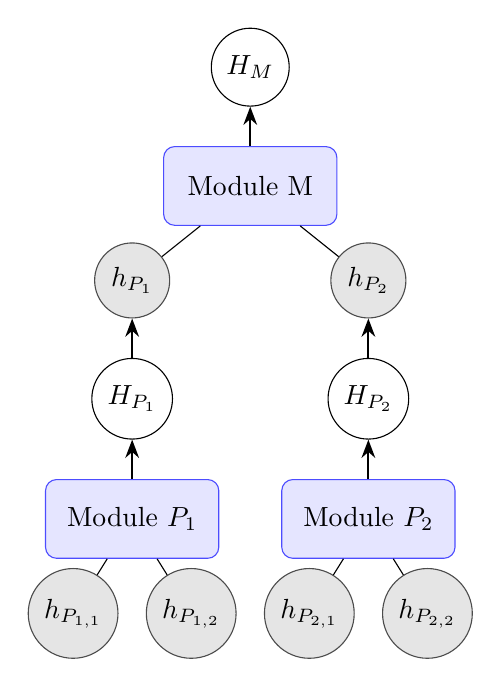
\begin{tikzpicture}[
	module/.style={rectangle, draw=blue!70, fill=blue!10, rounded corners, minimum width=2.2cm, minimum height=1cm},
	leaf/.style={circle, draw=black!70, fill=gray!20, minimum size=0.8cm},
	internal/.style={circle, draw=black, fill=white, minimum size=0.8cm},
	arrow/.style={-Stealth, thick},
	level distance=1.2cm, sibling distance=2.2cm
]

% Top-level module
\node[module] (M) {Module M}
	[sibling distance=3cm]
	child { node[leaf] (L1) {$h_{P_1}$} }
	child { node[leaf] (L2) {$h_{P_2}$} }
;

% Internal hash of M
\node[internal] (Root) [above=0.5cm of M] {$H_M$};
\draw[arrow] (M) to (Root);

\node[internal] (H1) [below=0.5cm of L1] {$H_{P_1}$};

% Parent 1's own subtree
\node[module] (P1) [below=0.5cm of H1] {Module $P_1$}
	[sibling distance=1.5cm]
	child { node[leaf] (L11) {$h_{P_{1,1}}$} }
	child { node[leaf] (L12) {$h_{P_{1,2}}$} }
;
\draw[arrow] (P1) to (H1);
\draw[arrow] (H1) to (L1);

\node[internal] (H2) [below=0.5cm of L2] {$H_{P_2}$};
% Parent 2's own subtree
\node[module] (P2) [below=0.5cm of H2] {Module $P_2$}
	[sibling distance=1.5cm]
	child { node[leaf] (L21) {$h_{P_{2,1}}$} }
	child { node[leaf] (L22) {$h_{P_{2,2}}$} }
;
\draw[arrow] (P2) to (H2);
\draw[arrow] (H2) to (L2);
\end{tikzpicture}
\caption{Recursive Merkle-tree inheritance: each module's finalized hash $H_{P_i}$ (shown as an internal node) is itself a Merkle root over its own parents, and these hashes become the leaves of its child's tree.}
\label{fig:recursive-merkle}
\Description[Recursive Merkle-tree inheritance.]{Recursive Merkle-tree inheritance: each module's finalized hash H_{P_i} (shown as an internal node) is itself a Merkle root over its own parents, and these hashes become the leaves of its child's tree.}
\end{figure}

\begin{figure}[t]
\centering
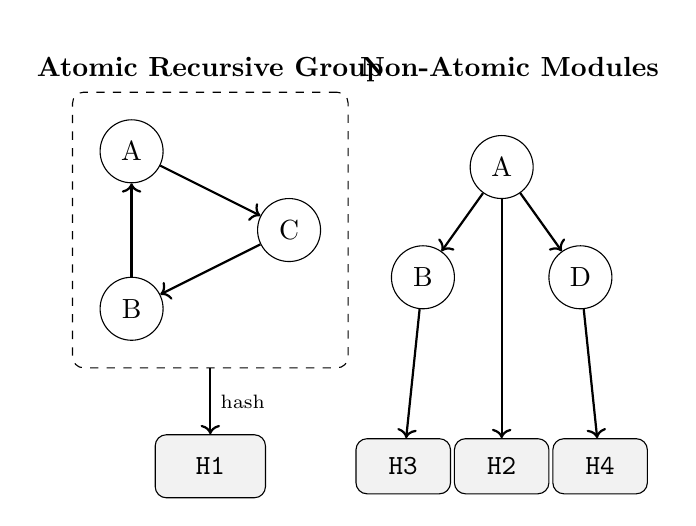
\begin{tikzpicture}[
	module/.style={circle,draw,minimum size=8mm,inner sep=0pt},
	hashbox/.style={rectangle,draw,dashed,rounded corners,inner sep=6pt},
	arrow/.style={->,thick}
]

% Atomic Recursive Module
\node[hashbox, minimum width=3.5cm, minimum height=3.5cm, label=above:{\textbf{Atomic Recursive Group}}] (g1) at (0,0) {};
\node[module] (A) at (-1,1) {A};
\node[module] (B) at (-1,-1) {B};
\node[module] (C) at (1,0) {C};

\draw[arrow] (A) -- (C);
\draw[arrow] (C) -- (B);
\draw[arrow] (B) -- (A);

% Hash arrow
\node[draw=none] (plus) at (2.2,0) {};
\node[draw,rectangle,rounded corners,fill=gray!10,minimum width=1.4cm,minimum height=0.8cm] (h1) at (0,-3) {\texttt{H1}};
\draw[arrow] (g1.south) -- (h1.north) node[midway,right] {\scriptsize hash};

% Non-Atomic Modules
\node[rectangle, draw=none, minimum height=1cm] (label2) at (3.8,2.07) {\textbf{Non-Atomic Modules}};
\node[module] (D) at (3.7,0.8) {A};
\node[module] (E) at (2.7,-0.6) {B};
\node[module] (F) at (4.7,-0.6) {D};

\draw[arrow] (D) -- (E);
\draw[arrow] (D) -- (F);

% Hashes
\node[draw,rectangle,rounded corners,fill=gray!10,minimum width=1.2cm,minimum height=0.7cm] (hD) at (3.7,-3) {\texttt{H2}};
\node[draw,rectangle,rounded corners,fill=gray!10,minimum width=1.2cm,minimum height=0.7cm] (hE) at (2.45,-3) {\texttt{H3}};
\node[draw,rectangle,rounded corners,fill=gray!10,minimum width=1.2cm,minimum height=0.7cm] (hF) at (4.95,-3) {\texttt{H4}};

\draw[arrow] (E) -- (hE);
\draw[arrow] (F) -- (hF);
\draw[arrow] (D) -- (hD);

\end{tikzpicture}
\caption{Atomic recursive modules are grouped and hashed as a single unit (\texttt{H1}), while non-atomic modules are hashed individually (\texttt{H2}, \texttt{H3}, \texttt{H4}).}
\label{fig:recursive-vs-nonrecursive}
\Description{Atomic recursive modules are grouped and hashed as a single unit (H1), while non-atomic modules are hashed individually (H2, H3, H4). The diagram shows 3 atomic recursive modules and 3 non-atomic modules.}
\end{figure}

\section{Use Cases and Interoperability}

This section illustrates how Merkle tree-based inheritance enables both fine-grained overrides and seamless integration with existing ecosystems.

\subsection{Overriding and Forking a Dependency}
Suppose a developer depends on a module \texttt{libA} that exports a function \texttt{validate()}. Traditionally, patching \texttt{validate()} requires forking the entire package and updating downstream dependencies. With Merkle inheritance, the developer creates a new module \texttt{libB}:

\begin{lstlisting}[language=json, basicstyle=\ttfamily\small,caption={Override of \texttt{validate()} in a new module}]
{
  % libA's finalized hash
  "imports": ["merkle:abcd...1234"],
  "exports": {
    "validate": /* new implementation */
  }
}
\end{lstlisting}

\noindent During finalization, \texttt{libB} reuses all symbols from \texttt{libA} except \texttt{validate}. Clients can verify this override by inspecting the Merkle ancestry proof. Figure~\ref{fig:module-resolution} illustrates conflict resolution rules in a similar context.

\subsection{Semver Translation Workflow}
Many projects declare dependencies with semver ranges (e.g.\ ``\verb|^1.3.0|'' in npm or Cargo). To interoperate, an import adapter resolves these ranges against the native ecosystem registry, then replaces them with concrete Merkle roots:

\begin{enumerate}
	\item Read \texttt{package.json} or \texttt{Cargo.toml}.
	\item Use npm/Cargo to select version \texttt{1.3.5}.
	\item Query the Merkle registry: 
		\[
			(\texttt{libA},1.3.5) \xrightarrow{\mathcal{R}} \texttt{merkle:abcd...1234}.
		\]
	\item Rewrite imports to \texttt{merkle:abcd...1234} before finalization.
\end{enumerate}

This workflow yields lockfile-free, content-addressed builds that remain reproducible.

\subsection{Runtime Symbol Resolution}
At execution time, symbols are resolved lazily via a \texttt{Resolver} class (Listing~\ref{fig:lazy-resolution}). The runtime consults a static reference map and fetches modules on demand. Figure~\ref{fig:interactive-resolution} diagrams this process.

\subsection{Registry Integration}
A decentralized registry maps human-readable names and version constraints to Merkle roots:
\[
\mathcal{R} : (\texttt{namespace},\texttt{name},\texttt{semver}) \;\mapsto\; h_M.
\]
Clients verify digital signatures on namespace Merkle roots to ensure only authorized publishers can update entries. This design supports:
\begin{itemize}
	\item \emph{Exact-version lookup}, ensuring reproducibility.
	\item \emph{Alternative registries}, allowing private or mirrored namespaces.
	\item \emph{Auditability}, via signed Merkle proofs of registry bindings.
\end{itemize}

\section{Merkle Tree-Based Inheritance Model}
\label{sec:merkle-inheritance}

I now present the core inheritance model built on Merkle trees and content addressing. Each module's direct parent hashes already embed their full ancestry, so finalization need only rehash those parent IDs.

\subsection{Merkle Trees}
A Merkle tree is a binary hash tree in which each leaf is the hash of a data element and each internal node is the hash of its two children. This enables:
\begin{itemize}
	\item \emph{Efficient inclusion proofs}, via logarithmic-sized authentication paths.
	\item \emph{Tamper detection}, since any change to a leaf or subtree propagates to the root.
\end{itemize}

\subsection{Content-Addressed Modules}
Each module $M$ consists of content $C_M$ and a (possibly empty) set of symbolic imports $I_M$. Modules are identified by:
\[
	h_C = H(C_M),
	\qquad
	h_M = H\bigl(h_C \,\|\, H_{\mathit{merkle}}(P)\bigr),
\]
where $P$ is the set of finalized parent hashes. Because each parent hash $h_{P_i}$ already encodes its own ancestry, hashing $P$ suffices to capture the entire transitive closure. As shown in Figure \ref{fig:recursive-merkle}, each parent hash $H_{P_i}$ is itself computed by hashing its own parents, and then is used as a leaf in module $M$'s tree.

\subsection{Inheritance Mechanism}
To inherit from parent modules:
\begin{enumerate}
	\item Resolve each import $i\in I_M$ via the registry \\$\mathcal{R}(i)\mapsto h_{P_i}$.
	\item Collect direct parents $P = \{h_{P_1},\dots,h_{P_k}\}$.
	\item Sort $P$ lexicographically and build a balanced \\Merkle tree to compute
		\[
			m = H_{\mathit{merkle}}(P).
		\]
	\item Compute the final ID
		\[
			h_M = H\bigl(h_C \,\|\, m\bigr).
		\]
\end{enumerate}

\subsection{Canonicalization of Ancestry}
Since each $h_{P_i}$ is itself a Merkle root over its parents, this process efficiently and deterministically captures all transitive ancestors without explicit recursion. The final module ID $h_M$ is a hash of both the content and the Merkle tree of its parents, ensuring that any change to $M$ or its ancestors yields a different $h_M$. This guarantees reproducibility and integrity. Figure \ref{fig:recursive-merkle} illustrates the recursive nature of this inheritance model.

\subsection{Symbol Resolution Semantics}
I view symbol resolution as a total function over the Merkle DAG: shadowing and override precedence follow a deterministic, breadth-first merge of ancestors. Each lookup records a symbolic trace of visited modules, making conflict resolution transparent and analyzable~\cite{dreyer2003typesystem,ancona2003foundations}. Formal judgments and proofs of soundness and determinism appear in the next section.

\subsection{Atomic Recursive Modules and Resolution Edge Cases}

The module system is built on Merkle tree-based inheritance, where each module is identified by a cryptographic hash of its resolved contents. This ensures reproducibility, immutability, and safe composition. To support recursive structures within this framework, we introduce the concept of \emph{atomic recursive modules}, which allow internally self-referential definitions without violating the acyclic nature of the Merkle graph.

\subsubsection{Recursive Modules via Atomic Grouping}
\label{sec:recursive-modules}

In standard Merkle tree semantics, recursive definitions pose a challenge because a module cannot refer to itself directly as doing so would prevent computing its hash. To address this, recursive modules are treated as \emph{atomic groups}: instead of resolving definitions incrementally, the entire group is resolved as a single unit and hashed only after all internal references are finalized.

This allows the system to support recursive structures like trees, lists, and graphs. For example, a binary tree can be defined recursively using a self-referential module that is resolved atomically (see subsection \ref{sec:worked-example-tree}). The atomic group ensures that all internal references are scoped and validated together, preventing any external circular dependencies.

While modules within an atomic group may reference each other recursively, the group as a whole is finalized before it can be linked elsewhere. This preserves the global acyclicity of the Merkle dependency graph. Any cycle involving multiple atomic groups is rejected at resolution time.

\subsubsection{Conflicting Module Versions}
\label{sec:conflicting-versions}

Conflicting versions of a dependency often lead to ambiguity or runtime bugs in traditional systems. Here, version conflicts are handled cleanly through content-addressing. Because each module version yields a different hash, they are treated as distinct modules by the system.

Multiple versions of a module can be imported and used independently:

\begin{quote}
	\texttt{import "crypto@1.2.0" as crypto\_v1;}\\
	\texttt{import "crypto@2.0.1" as crypto\_v2;}
\end{quote}

These modules coexist safely: their hashes, scope, and contents are isolated, and the system performs no implicit merging. When compiled to sandboxed targets like WebAssembly, their runtime separation is further enforced at the memory and execution boundary.

Tools can analyze the Merkle graph to report redundant or shadowed versions, but this is an opt-in ergonomic aid. The underlying resolution remains deterministic and transparent: different hashes mean different modules, regardless of name similarity or structural overlap.

\paragraph{Summary.}
Atomic recursive modules make recursive definitions first-class citizens within a Merkle tree-based module system. They preserve the resolution guarantees of immutability and acyclic structure, while enabling the expressive power needed for self-referential data types and algorithms. At the same time, versioning remains unambiguous and composable, supporting robust modular reuse in large and complex systems.

\subsection{Worked Example: Symbol Resolution and Override Tracing}

To demonstrate how finalization and symbol resolution interact with override tracing, consider the following module hierarchy:

\begin{lstlisting}[caption=Module definitions for resolution example]
module A {
  val x = 1
  val y = 2
}

module B inherits A {
  val y = 3
  val w = x + y
}

module C inherits A {
  val z = y + 10
}

module D inherits B, C {
  val u = z + w
}
\end{lstlisting}

Finalization proceeds bottom-up:

\begin{itemize}
	\item Module \texttt{A} has no parents and is finalized first.
	\item Module \texttt{B} inherits from \texttt{A}, overrides \texttt{y}, and defines \texttt{w}.
	\item Module \texttt{C} also inherits from \texttt{A}, reuses \texttt{y}, and defines \texttt{z}.
	\item Module \texttt{D} inherits from both \texttt{B} and \texttt{C}, and defines \texttt{u}.
\end{itemize}

When resolving the symbol \texttt{u} in \texttt{D}, the override trace proceeds as follows:

\begin{itemize}
	\item \texttt{u} depends on \texttt{z} and \texttt{w}.
	\item \texttt{z} is defined in \texttt{C}, which inherits \texttt{y} from \texttt{A}, so \texttt{z} resolves to $2 + 10 = 12$.
	\item \texttt{w} is defined in \texttt{B} and depends on \texttt{x} and the overridden \texttt{y}, so \texttt{w} resolves to $1 + 3 = 4$.
	\item \texttt{u} therefore resolves to $12 + 4 = 16$.
\end{itemize}

The trace for \texttt{u} shows multiple inheritance paths and captures symbol provenance:

\[
\texttt{u} \mapsto \texttt{z} + \texttt{w} \Rightarrow
\begin{cases}
	\texttt{z} \in \texttt{C} \Rightarrow \texttt{y} \in \texttt{A} \\
	\texttt{w} \in \texttt{B} \Rightarrow \texttt{x} \in \texttt{A}, \texttt{y} \text{ overridden in } \texttt{B}
\end{cases}
\]

This trace confirms:
\begin{itemize}
	\item Deterministic symbol resolution even in the presence of overrides.
	\item Accurate ancestry mapping via finalized hashes.
	\item That override points are explicitly captured in the trace.
\end{itemize}

The finalized hash of module \texttt{D} includes the finalized hashes of both \texttt{B} and \texttt{C}, recursively covering the full ancestry tree. This enables cryptographic validation of symbol provenance and ensures deterministic rebuilds.

\begin{figure}[ht]
\centering
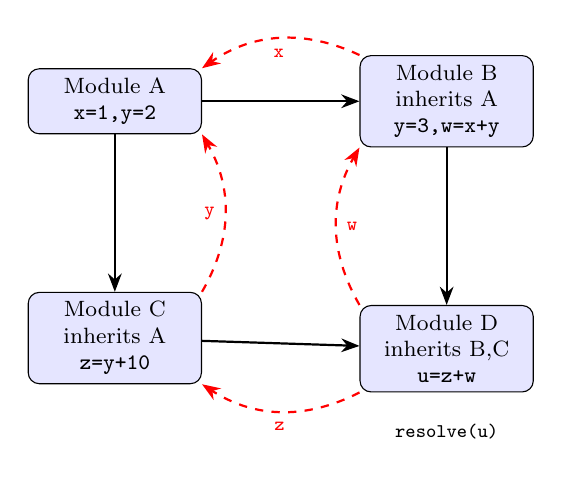
\begin{tikzpicture}[
	module/.style={rectangle, draw=black, rounded corners, fill=blue!10, minimum width=2.2cm, minimum height=0.8cm, font=\footnotesize, align=center},
	arrow/.style={-Stealth, thick},
	resolve/.style={dashed, red, -Stealth, thick}
]

% Modules
\node[module] (A) {Module A\\\texttt{x=1,y=2}};
\node[module, right=of A, xshift=1cm] (B) {Module B\\inherits A\\\texttt{y=3,w=x+y}};
\node[module, below=of A, yshift=-1cm] (C) {Module C\\inherits A\\\texttt{z=y+10}};
\node[module, below=of B, yshift=-1cm] (D) {Module D\\inherits B,C\\\texttt{u=z+w}};

% Inheritance arrows
\draw[arrow] (A) -- (B);
\draw[arrow] (A) -- (C);
\draw[arrow] (B) -- (D);
\draw[arrow] (C) -- (D);

% Resolution paths for u
\coordinate (u) at ($(D.south)+(0,-0.5)$);
\node at (u) [font=\scriptsize] {\texttt{resolve(u)}};

% dashed resolution arrows
\draw[resolve] (D.south west) to[bend left]  
	node[midway,below,font=\scriptsize]{\texttt{z}}
	(C.south east);
\draw[resolve] (D.north west) to[bend left]
	node[midway,right,font=\scriptsize]{\texttt{w}}
	(B.south west);

% Further resolution: z -> C -> A.y
\draw[resolve] (C.north east) to[bend right]
	node[midway,left,font=\scriptsize]{\texttt{y}}
	(A.south east);
% Further resolution: w -> B -> A.x
\draw[resolve] (B.north west) to[bend right]
	node[midway,below,font=\scriptsize]{\texttt{x}}
	(A.north east);

\end{tikzpicture}
\caption{Symbol resolution for \texttt{u} in Module D. Solid arrows show inheritance; dashed red arrows trace how \texttt{u = z + w} resolves through \texttt{z} in C (then \texttt{y} in A) and \texttt{w} in B (then \texttt{x} in A).}
\label{fig:resolution-example}
\Description[Symbol resolution for \texttt{u} in Module D.]{Symbol resolution for \texttt{u} in Module D. Solid arrows show inheritance; dashed red arrows trace how \texttt{u = z + w} resolves through \texttt{z} in C (then \texttt{y} in A) and \texttt{w} in B (then \texttt{x} in A).}
\end{figure}

Figure~\ref{fig:resolution-example} illustrates how the symbol \texttt{u} in Module D is resolved:

1. D inherits from B and C.
2. The dashed red arrow from D to C shows that \texttt{z} is looked up in C, which in turn inherits \texttt{y} from A.
3. The dashed red arrow from D to B shows that \texttt{w} is looked up in B, which uses the overridden \texttt{y} from B and \texttt{x} from A.
4. Ultimately, \texttt{u = z + w} resolves to values computed from A's and B's definitions, and the Merkle finalization of D incorporates the finalized hashes of B and C (which themselves embed A), ensuring full transitive integrity.

\subsection{Worked Example: A Recursive Module for Binary Trees}
\label{sec:worked-example-tree}

Recursive modules are essential for defining tree-like structures, where each node can contain subtrees of the same type. In this example, we use a recursive module to define a binary tree of integers.

\paragraph{Module Definition.}
We define a module named \texttt{tree} that contains a class \texttt{Tree}. This class represents either a \texttt{Leaf}, or a \texttt{Node} containing an integer value and two child trees.

\begin{verbatim}
# Module: tree
class Leaf:
	pass

class Node:
	def __init__(
			self,
			value: int,
			left: 'Tree',
			right: 'Tree'
		):
		self.value = value
		self.left = left
		self.right = right

Tree = Leaf | Node
\end{verbatim}

This structure is recursive: a \texttt{Node} refers to instances of \texttt{Tree}, which can themselves be \texttt{Node}s or \texttt{Leaf}s.

\paragraph{Example Construction.}
Here is how we can construct a simple binary tree with three nodes:

\begin{verbatim}
t = Node(1,
		 Node(2, Leaf(), Leaf()),
		 Node(3, Leaf(), Leaf()))
\end{verbatim}

\paragraph{Visual Representation.}
The structure of this tree can be visualized as follows:

\begin{center}
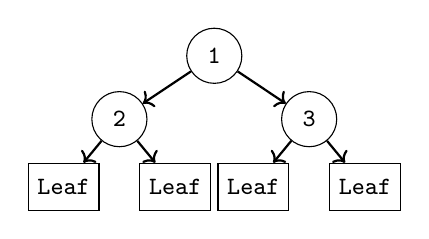
\begin{tikzpicture}[
	font=\ttfamily\small,
	rootnode/.style={draw, circle, minimum size=7mm},
	treenode/.style={draw, circle, minimum size=7mm, node distance=3mm and 7mm},
	leafnode/.style={draw, rectangle, minimum size=6mm, node distance=3mm and 0mm},
	pointer/.style={->, thick}
]

\node[rootnode] (root) {1};
\node[treenode, below left=of root] (left) {2};
\node[treenode, below right=of root] (right) {3};
\node[leafnode, below left=of left] (l1) {Leaf};
\node[leafnode, below right=of left] (l2) {Leaf};
\node[leafnode, below left=of right] (r1) {Leaf};
\node[leafnode, below right=of right] (r2) {Leaf};

\draw[pointer] (root) -- (left);
\draw[pointer] (root) -- (right);
\draw[pointer] (left) -- (l1);
\draw[pointer] (left) -- (l2);
\draw[pointer] (right) -- (r1);
\draw[pointer] (right) -- (r2);

\end{tikzpicture}
\end{center}

\paragraph{Recursive Rule.}
With the recursive structure in place, we can define a recursive function to count the number of nodes in the tree:

\begin{verbatim}
def size(t: Tree) -> int:
	if isinstance(t, Leaf):
		return 0
	elif isinstance(t, Node):
		return 1 + size(t.left) + size(t.right)
\end{verbatim}

This function uses standard Python-style pattern \\matching with \texttt{isinstance}, and recursively counts all the internal \texttt{Node}s in the tree.

\paragraph{Summary.}
This example illustrates how recursive data structures can be implemented cleanly using modules. By using classes to define variants like \texttt{Leaf} and \texttt{Node}, and recursive references to the type \texttt{Tree}, we can express complex hierarchical data naturally.

\section{Formal Module Semantics}
\label{sec:formal-semantics}

This section states the key judgments, inference rules, and metatheoretic properties of symbol resolution and override traces.

\subsection{Resolution Judgments and Inference Rules}
\[
	M \vdash s \Downarrow d
	\quad\text{and}\quad
	M \vdash s \Downarrow d \leadsto \pi
\]
where $\pi$ is the override trace. The rules are:

\mprset{flushleft}
\begin{mathpar}
\inferrule
{s \in \mathrm{dom}(\Gamma_M) \\ \Gamma_M(s) = d}
{M \vdash s \Downarrow d}
\quad\textsc{(Local)}

\inferrule
{P_i \vdash s \Downarrow d \\ \forall j < i.\; s \notin \mathrm{dom}(\Gamma_{P_j})}
{M \vdash s \Downarrow d}
\quad\textsc{(Inherit)}
\end{mathpar}

\begin{mathpar}
\inferrule
{s \in \mathrm{dom}(\Gamma_M)}
{M \vdash s \Downarrow d \leadsto [M]}
\quad\textsc{(T-Loc)}

\inferrule
{P_i \vdash s \Downarrow d \leadsto \pi \\ \forall j < i.\; s \notin \mathrm{dom}(\Gamma_{P_j})}
{M \vdash s \Downarrow d \leadsto [M] \mathbin{++} \pi}
\quad\textsc{(T-Inh)}
\end{mathpar}

\subsection{Metatheoretic Properties}

\paragraph{Determinism.} 
\emph{Theorem.} If $M \vdash s \Downarrow d_1$ and $M \vdash s \Downarrow d_2$, then $d_1 = d_2$.

\paragraph{Typing Judgment (Sketch).} 
Each module $M$ has a typing context $\Gamma_M$. I write
\[
	\Gamma \vdash M : \mathsf{OK}
\]
to mean all definitions and references in $M$ are type-consistent. Child overrides may freely redefine types; consumers of $M$ perform verification upon import.

\paragraph{Soundness, Compositionality.} 
Resolution is sound (every resolved symbol is a valid definition), compositional (combining DAG fragments preserves resolution outcomes), and deterministic (no nondeterminism in lookup). Detailed proofs are in the appendix.

\subsection{Worked Formal Example}
\label{sec:worked-formal-example}

We illustrate the formal resolution judgment
\[
	M \vdash s \Downarrow d \leadsto \pi
\]
using the modules from our worked example:

\begin{itemize}
	\item $A$ exports $\{x,y\}$.
	\item $B$ inherits $A$ and overrides $y$.
	\item $C$ inherits $A$ without overrides.
	\item $D$ inherits $B,C$.
\end{itemize}

We show the derivation of
\[
  D \vdash x \Downarrow (A,x) \leadsto [D,B,A]\,
\]
using rules \textsc{T-Loc} and \textsc{T-Inh}:

\begin{mathpar}
\inferrule[T-Loc-A]{
  x \in \mathit{dom}(\Gamma_A) \\
  \Gamma_A(x) = (A,x)
}{
  A \vdash x \Downarrow (A,x) \leadsto [A]
}
\end{mathpar}

\begin{mathpar}
\inferrule[T-Inh-B]{
  A \vdash x \Downarrow (A,x) \leadsto [A] \\
  \forall j < 1,\; x \notin \mathit{dom}(\Gamma_{P_j})
}{
  B \vdash x \Downarrow (A,x) \leadsto [B] \mathbin{++} [A]
}
\end{mathpar}

\begin{mathpar}
\inferrule[T-Inh-D]{
  B \vdash x \Downarrow (A,x) \leadsto [B,A] \\
  \forall j < 1,\; x \notin \mathit{dom}(\Gamma_{C})
}{
  D \vdash x \Downarrow (A,x) \leadsto [D] \mathbin{++} [B,A]
}
\end{mathpar}


Here:
\begin{itemize}
	\item Rule \textsc{T-Loc-A} applies in $A$ since $x$ is locally defined.
	\item Rule \textsc{T-Inh-B} lifts the result into $B$, skipping over any earlier parents that do not define $x$.
	\item Rule \textsc{T-Inh-D} finally lifts into $D$, yielding the full override trace $\pi = [D,B,A]$.
\end{itemize}

This derivation demonstrates:
\begin{enumerate}
	\item \emph{Determinism}: each step picks the first ancestor defining $x$.
	\item \emph{Trace capture}: the list $[D,B,A]$ records the chain of modules visited.
	\item \emph{Compositionality}: resolution in $D$ reuses the \\derivation in $B$.
\end{enumerate}

\section{Lean Theorems}
\label{sec:lean-theorems}

I state the core properties of the Merkle hashing and override-trace mechanisms.  Full mechanized proofs appear in Appendix~\ref{supp-appendix:formal-proofs}.

\begin{theorem}[Deterministic Merkle Hashing]
\label{thm:treeHash_deterministic}
For any sorted list of hashes \(L\), all balanced Merkle-tree constructions over \(L\) yield the same root:
\[
	\forall\,T_1, T_2.\quad
		\mathit{treeHash}_{T_1}(L) \;=\; \mathit{treeHash}_{T_2}(L).
\]
\end{theorem}
\noindent\emph{Proof sketch.}  Both constructions only reorder and hash pairs of elements in \(L\), and SHA-256 is collision-resistant.  See Appendix~\ref{supp-appendix:determinism} for the full proof.

\begin{lemma}[List-to-Tree Correctness]
\label{lem:listToTree_correctness}
For any sorted list \(L\),
\[
	\mathit{leaves}\bigl(\mathit{listToTree}(L)\bigr) \;=\; L.
\]
\end{lemma}
\noindent\emph{Proof sketch.}  By induction on the balanced-tree construction function, which preserves input order at the leaves.  See Appendix~\ref{supp-appendix:injectivity}.

\begin{theorem}[Compositional Merkle Hash]
\label{thm:merkleHash_compositional}
For any two (possibly overlapping) sets of parent hashes \(P_1\) and \(P_2\),
\[
	H_{\mathit{merkle}}(P_1 \cup P_2)
		= H\bigl(H_{\mathit{merkle}}(P_1)\,\|\,
			H_{\mathit{merkle}}(P_2)\bigr).
\]
\end{theorem}
\noindent\emph{Proof sketch.}  Shared elements appear exactly once in the union and in both subtrees; merging two roots preserves the canonical structure.  See Appendix~\ref{supp-appendix:monotonicity}.

\begin{proposition}[Override Trace Finiteness]
\label{prop:overrideTrace_properties}
For every symbol \(s\) in a finalized module, its override trace \(\pi = \mathrm{trace}(s)\) is a finite, acyclic sequence of module IDs.
\end{proposition}
\noindent\emph{Proof sketch.}  Cycles are impossible because each group or module is frozen before hashing, and the import graph is collapsed to a DAG of atomic nodes.  See Appendix~\ref{supp-appendix:termination}.

\section{Formalization of Finalization}
\label{sec:formalization-finalization}

Before computing Merkle roots, the system first collapses any mutually recursive modules into atomic \\groups. Formally:

\begin{enumerate}
	\item \textbf{SCC collapse.} Given the symbolic import graph, compute its strongly-connected components \\(SCCs). Treat each SCC \(G\) as a single atomic node whose content is the canonical serialization of all modules in \(G\).
	\item \textbf{Resolve imports.} For each remaining symbolic reference \(r\), look up its finalized parent hash \(h_{P} = \mathcal{R}(r)\), where \(P\) includes both standalone modules and atomic groups.
	\item \textbf{Collect direct parents.} Let
	\[
		P = \{h_{P_1}, \dots, h_{P_k}\}.
	\]
	Each \(h_{P_i}\) already encodes its own transitive ancestry (and any recursion is contained within its atomic group).
	\item \textbf{Compute parent Merkle root.} Sort \(P\) lexicographically and build a balanced Merkle tree; let
	\[
		m = H_{\mathit{merkle}}(P).
	\]
	\item \textbf{Content hash.} Compute
	\[
		h_C = H(C_M).
	\]
	\item \textbf{Final module ID.} Return
	\[
		h_M = H\bigl(h_C \,\|\, T_M \,\|\, A_M \,\|\, m\bigr).
	\]
\end{enumerate}

This procedure remains fully static and deterministic. By collapsing recursive groups before hashing, we preserve an acyclic DAG for Merkle-tree finalization while still supporting mutual recursion internally.

\paragraph{Key Property.} 
Since each direct parent hash $h_{P_i}$ already encodes its full ancestry, step 3 suffices to guarantee that $h_M$ reflects all transitive ancestors without needing an explicit closure computation.

\subsection{Determinism and Injectivity}
\paragraph{Determinism.} 
Repeated application of $\mathcal{F}$ on the same inputs yields the same $h_M$, since all operations (registry lookup, sorting, hashing) are deterministic.

\paragraph{Injectivity.} 
If $\mathcal{F}(X_1)=\mathcal{F}(X_2)$ then $X_1=X_2$, by collision resistance of $H$ and inclusion of all distinguishing components ($C,T,A,P$) in the final hash.
\begin{figure}[tb]
\centering
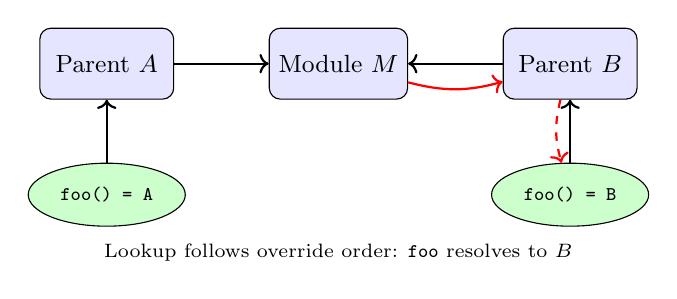
\begin{tikzpicture}[
	node distance=1.2cm and 1.2cm,
	module/.style={rectangle, draw=black, rounded corners, minimum width=1.7cm, minimum height=0.9cm, fill=blue!10, font=\small},
	symbol/.style={ellipse, draw=black, fill=green!20, minimum width=1.4cm, minimum height=0.8cm, font=\scriptsize},
	edge/.style={->, thick},
	rededge/.style={->, thick, red},
	dashededge/.style={->, dashed, thick, gray}
]

% Nodes
\node[module] (M) at (0,0) {Module $M$};
\node[module] (A) [left=of M] {Parent $A$};
\node[module] (B) [right=of M] {Parent $B$};

\node[symbol] (defA) [below=0.8cm of A] {\texttt{foo() = A}};
\node[symbol] (defB) [below=0.8cm of B] {\texttt{foo() = B}};

% Inheritance edges
\draw[edge] (A) -- (M);
\draw[edge] (B) -- (M);

% Definition edges
\draw[edge] (defA) -- (A);
\draw[edge] (defB) -- (B);

% Resolution path
\draw[rededge] (M) to[bend right=15] (B);
\draw[rededge, dashed] (B) to[bend right=15] (defB);

% Legend
\node[align=center, font=\scriptsize] at (0, -2.4) {Lookup follows override order: \texttt{foo} resolves to $B$};

\end{tikzpicture}
\caption{
Symbol resolution in a Merkle-based inheritance graph. Module $M$ inherits from parents $A$ and $B$, with left-to-right override precedence. The arrows illustrate the path taken to resolve the symbol \texttt{foo}, which is found in both parents. Dotted red arrows represent resolution from the module to the symbol definition.
}
\Description{Symbol resolution in a Merkle-based inheritance graph. Module M inherits from parents A and B, with left-to-right override precedence. Modules A and B each define a function foo that returns A and B, respectively. Module M resolves foo to module B's version because of the override precedence.}
\label{fig:semantics}
\end{figure}

\section{Type System Integration}
\label{sec:type-system-integration}

While the system remains fundamentally language-agno\-stic, many modern ecosystems rely on type annotations and interface contracts to ensure safe composition. To support this, I propose a two-phase type integration model that preserves the flexibility of content-addressed inheritance while enabling static guarantees where needed.

\paragraph{Two-Phase Typing for Module Finalization}
I introduce a two-phase typing model designed to catch type mismatches early while maintaining the independence and reusability of individual modules:

\begin{enumerate}
	\item \textbf{Pre-Finalization Type Annotation Phase}: \\Each module may declare its own exports and expected imports using optional type signatures. These annotations serve as structural contracts and can be checked in isolation without resolving the entire inheritance graph. This phase supports ecosystem-specific type formats (e.g., TypeScript, Flow, Rust types).
	\item \textbf{Post-Finalization Resolution Phase}: Once the full inheritance graph is resolved and finalized, the system performs type unification, verifying that re-exports and overrides preserve declared types. Any mismatches or violations of declared type bounds can be caught during this phase, ensuring that the final module is type-safe.
\end{enumerate}

This approach preserves local reasoning for individual modules, enables partial type-checking during development, and supports eventual consistency and validation in the finalized view. It also avoids requiring global type inference, which may not be tractable across distributed registries.

\paragraph{Optional Typing During Module Resolution}
Typ\-ed ecosystems can optionally perform type compatibility checks at resolution time. This includes verifying that imported or overridden symbols maintain compatible types, checking for shadowing violations, and ensuring interface conformity for inherited modules.

\paragraph{Declarative Type Annotations}
Modules may provide inline or sidecar type annotations, allowing downstream tools or runtimes to validate that symbols match their declared types. For example, if \texttt{moduleA} exports a function \texttt{compute()} with signature \texttt{Int $\to$ Int}, any modules inheriting or re-exporting it must preserve this type unless explicitly widened or aliased.

\paragraph{Generic Type Support}
Typed ecosystems may adopt \emph{generic type aliases} and structural type constraints to define parametric modules or enforce interface-like requirements across inheritance trees. These mechanisms are sketched in Appendix~\ref{supp-appendix:generics} and align with the semantics of finalization and override resolution.

By enabling early detection of type mismatches and supporting structural compatibility guarantees, the system provides a pathway to scalable, decentralized type safety. This approach is particularly useful for ecosystems seeking to layer formal validation atop content-addressed distribution.

As discussed in Section~\ref{sec:limitations-future}, future work includes implementing richer type inference mechanisms, subtyping hierarchies, and generics-aware resolution, enabling even more robust type integration across distributed modules.

\paragraph{Connections to Module Calculi.}
My system is not itself a formal module calculus, but it draws on key ideas from foundational work on ML-style modules~\cite{ml_modules} and the mixin calculus~\cite{mixin_calculus}. In particular, it supports compositionality, deterministic symbol resolution, and (optionally) generic module interfaces. Detailed discussion of its relationship to these calculi, and the requirements for supporting features like higher-order modules and recursive types, is provided in the supplementary materials (Appendix~\ref{supp-appendix:module-calculi}).

\section{Namespace-Based Registry}
\label{sec:namespace-based-registry}

To facilitate human-readable and interoperable module references, I introduce a decentralized registry system that maps symbolic names and version constraints to Merkle-based module identities. This registry layer provides a structured namespace for modules while preserving the immutability and transparency of the underlying content-addressed architecture.

\subsection{Human-Readable Naming}

To enable discoverability and developer ergonomics, modules may be referred to by symbolic identifiers of the form:
\[
	\texttt{namespace/name@version}
\]

For example:
\[
	\texttt{core/math@1.0.0}
\]

These identifiers are resolved to finalized module hashes via a distributed registry system.

\subsection{Registry Semantics}

I define a registry as a mapping:
\[
	\mathcal{R}: (\texttt{namespace}, \texttt{name}, \texttt{semver}) \rightarrow h_M
\]

Each registry entry is a triple that maps a human-readable namespace and identifier and a semantic version constraint to a finalized module ID.

\subsection{Version Constraints}

The current system supports only \emph{exact versioning} for modules. Modules must be referenced using fully specified semantic versions, such as \texttt{core/math@1.2.3}

This ensures reproducibility and avoids ambiguity during resolution. Each version corresponds to a finalized module hash, and resolution is a direct lookup of that specific version in the distributed registry.

While this restriction simplifies caching, distribution, and verification, it limits the ability to express flexible or evolving dependencies. As future work, I plan to support more expressive version constraints, including:

\begin{itemize}
	\item Compatible Versions: \verb#@^1.2.0#
	\item Version Ranges: \texttt{>=1.0.0 <2.0.0}
\end{itemize}

These forms would require additional mechanisms for compatibility analysis, deterministic resolution, and finalization tracking across evolving module sets.
\subsection{Support for \texttt{latest} Tag in Module References}

To improve developer ergonomics during early development and testing, the system supports symbolic module references using a reserved \texttt{latest} tag. This tag acts as a placeholder for the most recent version of a module available at the time of resolution, determined using a combination of metadata (e.g., version numbers, timestamps) or registry-specific heuristics.

\paragraph{Pre-Finalization Semantics.}
The \texttt{latest} tag is resolved during the pre-finalization phase of module compilation or bundling. At this stage, all symbolic references are dereferenced to content-addressed identifiers (e.g., hashes), ensuring that the finalized module graph remains immutable and reproducible. This allows developers to write:

\begin{verbatim}
import utils from "example.org/lib@latest";
\end{verbatim}

\noindent which is resolved to:

\begin{verbatim}
import utils from "example.org/lib@1.2#hash";
\end{verbatim}

\noindent based on the state of the distributed registry or a pinned version map at the time of finalization.

\paragraph{Reproducibility and Pinning.}
To ensure builds remain deterministic, the resolution of \texttt{latest} must be pinned to a concrete content hash before module finalization. Once resolved, symbolic tags are no longer part of the module graph. Build systems and registries should retain a record of the mapping between symbolic tags and resolved identifiers to support reproducibility audits.

\paragraph{Limitations.}
Because the \texttt{latest} tag is inherently non-deterministic, its use is discouraged in finalized modules or published registries. It is intended for use in development workflows, rapid prototyping, and interactive environments such as REPLs or notebooks. Static analyzers and linters may issue warnings if \texttt{latest} appears in production code paths.

\paragraph{Related Features.}
The system may also support additional symbolic tags like \texttt{beta}, \texttt{stable}, or semver-compatible wildcards (e.g., \texttt{1.x}), resolved via similar mechanisms before finalization. All symbolic references must ultimately reduce to a content-addressed form to participate in the Merkle tree-based inheritance model.

\subsection{Immutable Bindings}

Once a registry entry is created, it is immutable. That is:
\[
	\mathcal{R}(n, m, v) = h_M \quad \text{is fixed for all time}
\]

This ensures that symbolic references remain stable and verifiable over time.

\subsection{Distributed Implementation}

The registry is implemented as a distributed store backed by the same DHT infrastructure used for module exchange~\cite{dht}. Each namespace is a signed collection of bindings, rooted by a Merkle tree~\cite{merkle1978}:
\[
	\texttt{namespace} \rightarrow H_{\text{merkle}}(\text{bindings})
\]

Each binding is a tuple:
\[
	(\texttt{name}, \texttt{version}, h_M)
\]

Namespaces may be published and updated only by owners who can sign new Merkle roots. Ownership is tracked via public key cryptography, and clients verify signatures before accepting updates.

\subsection{Integration with Finalization}

During module finalization, any symbolic parent reference of the form:
\begin{verbatim}
import core/math@1.0.0
\end{verbatim}
is resolved through the registry:
\[
	(\texttt{core}, \texttt{math}, \texttt{1.0.0}) \xrightarrow{\mathcal{R}} h_{M'}
\]

The resulting module ID $h_{M'}$ is inserted into the parent set $P$, and all symbolic names are replaced by cryptographic hashes. This process is deterministic and ensures that the final module ID is fully derived from immutable data.

\subsection{Registry Trust Model}

Registries do not require global trust. Clients are free to:
\begin{itemize}
	\item Pin specific hashes instead of using symbolic \\names.
	\item Use alternate or private registries for specific \\namespaces.
	\item Require signatures from known authors or authorities.
\end{itemize}

This flexibility allows the ecosystem to support both centralized and decentralized workflows while preserving verifiability.

\section{Runtime and Resolution Semantics}
\label{sec:runtime-resolution-semantics}

In Tangl, modules are compiled into a platform-indep\-endent format (e.g., WebAssembly or JavaScript) and executed in a virtual machine (VM). A finalized module is fully deterministic: it includes a content-addressed identifier, a static resolution table, and a record of its transitive ancestry. At execution time, this structure enables on-demand, verifiable, and reproducible behavior.

\subsection{Resolve Phase}

Rather than preloading all dependencies, the Tangl VM performs a \emph{resolve phase} prior to execution:

\begin{itemize}
	\item It traverses the module's resolution map $R_M$, \\which maps symbol names to ancestor modules and specific exports.
	\item For each module ID referenced in $R_M$, it checks whether the corresponding module is available locally or locates it in the distributed network.
	\item A resolution index $\rho: h_{M_i} \mapsto \text{location}$ is constructed, mapping content hashes to their resolvable location (e.g., a local path, cached artifact, or network URI).
\end{itemize}

No modules are actually fetched or loaded during this phase. Instead, the resolve phase ensures that all necessary modules are \textit{locatable}, enabling efficient runtime linking.

\subsection{Lazy Loading at Runtime}

Once resolution is complete, the module is executed with \emph{lazy loading} semantics:

\begin{itemize}
	\item Ancestor modules are not loaded upfront.
	\item When a symbol is first accessed during execution, the VM uses $R_M$ to determine which ancestor module it belongs to.
	\item If the ancestor has not yet been loaded, the VM consults $\rho$ to fetch, parse, and instantiate it on demand.
	\item Resolved exports are cached for subsequent use.
\end{itemize}

This strategy ensures minimal startup overhead, efficient caching, and deterministic behavior across environments.


\subsection{Symbol Resolution Example}

To illustrate the resolution logic, consider a module \texttt{Main} that inherits from two modules \texttt{A} and \texttt{B}, both of which export a symbol \texttt{foo}. Tangl's resolution map $R_M$ determines which export is used based on two factors:

\begin{itemize}
	\item \textbf{Import Order:} If both modules define the same symbol, the last one imported "wins" by default.
	\item \textbf{Import Granularity:} A symbol-specific import (e.g., \texttt{import(A.foo)}) takes precedence over \\whole-module imports.
\end{itemize}

\paragraph{Scenario 1: Whole-module imports, ordered B then A}

\begin{verbatim}
import(B);
import(A);
foo();
\end{verbatim}

Even though both \texttt{A} and \texttt{B} export \texttt{foo}, the reference map $R_{\texttt{Main}}$ resolves:

\[
	R_{\texttt{Main}}(\texttt{foo}) = \langle \texttt{A}, \texttt{foo} \rangle
\]

because \texttt{A} was imported after \texttt{B}, overriding its binding.

\paragraph{Scenario 2: Symbol-specific import.}

\begin{verbatim}
import(A.foo);
import(B);
foo();
\end{verbatim}

Even though \texttt{B} was imported later, the reference map gives priority to the symbol-specific import:

\[
	R_{\texttt{Main}}(\texttt{foo}) = \langle \texttt{A}, \texttt{foo} \rangle
\]

This allows developers to explicitly pin symbols to particular modules, regardless of the overall import order.

\paragraph{Scenario 3: No disambiguation provided.}

\begin{verbatim}
import(A);
import(B);
foo();
\end{verbatim}

This resolves to:

\[
	R_{\texttt{Main}}(\texttt{foo}) = \langle \texttt{B}, \texttt{foo} \rangle
\]

since \texttt{B} was the last module imported that provided \texttt{foo}. Had both modules been imported in the reverse order, the binding would change.

\paragraph{Summary.}

Tangl's resolution rules provide both predictability and flexibility:

\begin{itemize}
	\item The default rule is \textit{last-imported wins}.
	\item Symbol-specific imports override full-module imports.
	\item Resolution is captured statically in $R_M$, which is persisted in the finalization step and guarantees reproducibility across machines and time.
\end{itemize}

This allows Tangl programs to explicitly disambiguate conflicting definitions and avoid ambiguous resolution paths without resorting to runtime heuristics.

\begin{lstlisting}[language=Python,
	caption={Lazy symbol resolution in the \texttt{Resolver} class},
	label={fig:lazy-resolution},
	basicstyle=\scriptsize\ttfamily,
	keywordstyle=\ttfamily,
	emphstyle=\ttfamily,
	commentstyle=\ttfamily,
	stringstyle=\ttfamily,
	breaklines=true,
	breakindent=0pt,
	frame=single,
	columns=fullflexible,
	keepspaces=true,
	showstringspaces=false,
]
class Resolver:
def __init__(
		self,
		reference_map,
		content_store,
		fetch_from_network
	):
	# foo -> a29d...3c23
	self.reference_map = reference_map
	# Local content store
	self.cs = content_store
	# Fetch fn
	self.fetch = fetch_from_network
	# Memoized resolutions
	self.resolved_cache = {}

def resolve(self, symbol):
	if symbol in self.resolved_cache:
		return self.resolved_cache[symbol]
	if symbol not in self.reference_map:
		raise ResolutionError(f"{symbol} not found")
	hash_id = self.reference_map[symbol]
	if not self.cs.contains(hash_id):
		module_data = self.fetch(hash_id)
		self.cs.store(hash_id, module_data)
	module = self.cs.load(hash_id)
	self.resolved_cache[symbol] = module
	return module

resolver = Resolver(reference_map, content_store, network_fetch_fn)
foo_module = resolver.resolve('foo')
\end{lstlisting}

\begin{figure}[ht]
\centering
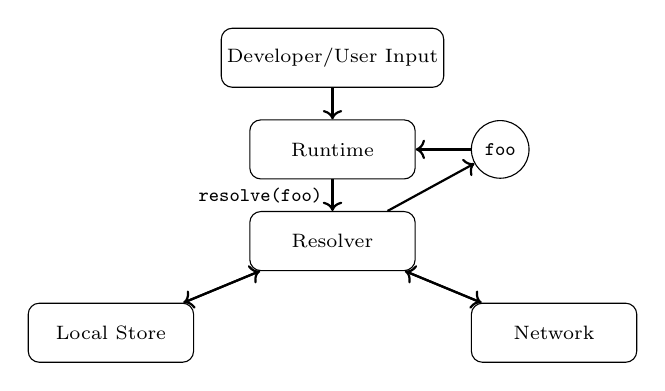
\begin{tikzpicture}[
	node distance=4mm and 7mm,
	font=\scriptsize,
	box/.style={draw, rounded corners, align=center, minimum width=2.1cm, minimum height=0.75cm, inner sep=2pt},
	arrow/.style={->, thick},
	sym/.style={circle, draw, minimum size=0.7cm, align=center}
]

% Nodes
\node[box] (dev) {Developer/User Input};
\node[box, below=of dev] (runtime) {Runtime};
\node[sym, right=of runtime] (foo) {\texttt{foo}};
\node[box, below=of runtime] (resolver) {Resolver};
\node[box, below left=of resolver] (local) {Local Store};
\node[box, below right=of resolver] (network) {Network};

% Edges
\draw[arrow] (dev) -- (runtime);
\draw[arrow] (runtime) -- (resolver) node[midway, left] {\texttt{resolve(foo)}};
\draw[arrow] (resolver) -- (local);
\draw[arrow] (resolver) -- (network);
\draw[arrow] (local) -- (resolver);
\draw[arrow] (network) -- (resolver);
\draw[arrow] (resolver) -- (foo);
\draw[arrow] (foo) -- (runtime);

\end{tikzpicture}
\caption{Runtime resolution of symbols like \texttt{foo} through local or network lookup.}
\Description{Runtime resolution of symbols like foo through local or network lookup. Resolution begins with developer or user input into the runtime. The runtime attempts to resolve foo through the resolver. The resolver uses the local store and/or the network to resolve foo and returns the appropriate symbol to the runtime.}
\label{fig:interactive-resolution}
\end{figure}

\subsection{Module Resolution Walkthrough}

To illustrate the module resolution process and how conflicts are handled, consider the following scenario involving two modules, \texttt{moduleA} and \texttt{moduleB}, both of which define a function \texttt{compute()}:

\begin{verbatim}
# moduleA.js
export function compute() { return 42; }

# moduleB.js
export function compute() { return 24; }
\end{verbatim}

A third module, \texttt{moduleC}, imports both \texttt{moduleA} and \texttt{moduleB}, and then calls \texttt{compute()}:

\begin{verbatim}
# moduleC.js
import { compute } from 'moduleA';
import { compute } from 'moduleB';

console.log(compute());
\end{verbatim}

Module resolution begins by evaluating imports in lexical order. In this case, the function \texttt{compute} from \texttt{moduleB} shadows the one from \texttt{moduleA} because it is imported later. Thus, \texttt{console.log(compute())} prints \texttt{24}, not \texttt{42}.

This rule, where later imports take precedence, is a key aspect of the system's lexical scoping model and ensures predictability: the most recently imported binding of a symbol is the one used.

\paragraph{Re-Exports.}

Now consider a re-export scenario \\where a module re-exports symbols from another:

\begin{verbatim}
# moduleA.js
export function compute() { return 42; }

# moduleB.js
export { compute } from 'moduleA';
export function compute() { return 24; }

# moduleC.js
import { compute } from 'moduleB';
console.log(compute());
\end{verbatim}

Here, \texttt{moduleB} re-exports \texttt{compute} from \texttt{moduleA}, but also defines its own version of \texttt{compute}. The local definition in \texttt{moduleB} takes precedence over the re-exported one, and so \texttt{console.log(compute())} prints \texttt{24}.

\paragraph{Nested Imports.}

Finally, consider a case with nested imports:

\begin{verbatim}
# base.js
export function compute() { return 1; }

# lib.js
import { compute as baseCompute } from 'base';
export function compute() {
	return baseCompute() + 1;
}

# app.js
import { compute } from 'lib';
console.log(compute());
\end{verbatim}

In this example, \texttt{lib.js} imports \texttt{compute} from \\\texttt{base.js} under the alias \texttt{baseCompute}, then defines its own \texttt{compute} that builds on it. When \texttt{app.js} imports from \texttt{lib.js}, it sees only the final \texttt{compute}—which returns \texttt{2}.

This demonstrates how symbol resolution in nested modules always respects lexical ordering and explicit rebinding: imported symbols are only visible where they are explicitly propagated.

\paragraph{Summary.}

These examples collectively illustrate \\how lexical import order and explicit rebindings guide name resolution. The "last import wins" rule ensures intuitive behavior while allowing developers to override or refine imported symbols as needed.

\subsection{Execution Model Summary}

Execution proceeds as follows:
\begin{enumerate}
	\item \textbf{Resolve:} Traverse $R_M$ to locate all ancestor modules by hash and build $\rho$.
	\item \textbf{Instantiate:} Load and prepare \texttt{Main} for execution with no parent modules yet loaded.
	\item \textbf{Evaluate:} As symbols are accessed, dynamically load ancestors and resolve symbols according to $R_M$.
\end{enumerate}

This model allows large dependency graphs to be traversed efficiently and on-demand, while maintaining strong guarantees of determinism, immutability, and verifiability.

\begin{figure}[t]
\centering
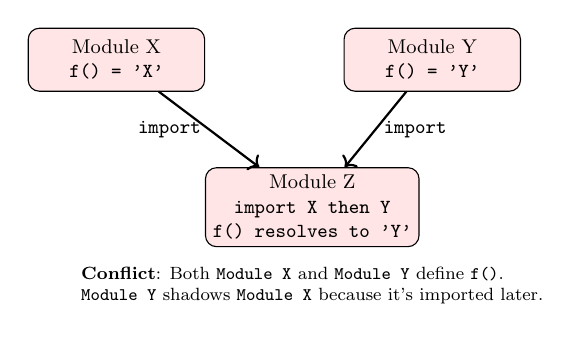
\begin{tikzpicture}[
	scale=0.8, transform shape,
	node distance=1.7cm and 2.2cm,
	every node/.style={font=\small},
	module/.style={rectangle, draw=black, fill=red!10, rounded corners, minimum width=2.8cm, minimum height=1cm, align=center},
	arrow/.style={->, thick}
]

% Modules for Conflict Scenario
\node[module] (modX) {Module X\\ \texttt{f() = 'X'}};
\node[module, right=of modX] (modY) {Module Y\\ \texttt{f() = 'Y'}};
\node[module, below right=1.2cm and 0cm of modX] (modZ) {Module Z\\ \texttt{import X then Y}\\ \texttt{f() resolves to 'Y'}};

% Arrows for Conflict Scenario
\draw[arrow] (modX) -- (modZ) node[midway, left] {\texttt{import}};
\draw[arrow] (modY) -- (modZ) node[midway, right] {\texttt{import}};

% Annotation for Conflict Scenario
\node[align=left, below=0.2cm of modZ, font=\footnotesize] {
\textbf{Conflict}: Both \texttt{Module X} and \texttt{Module Y} define \texttt{f()}.\\
\texttt{Module Y} shadows \texttt{Module X} because it's imported later.
};

\end{tikzpicture}

\vspace{1cm} % Add some space between the two diagrams

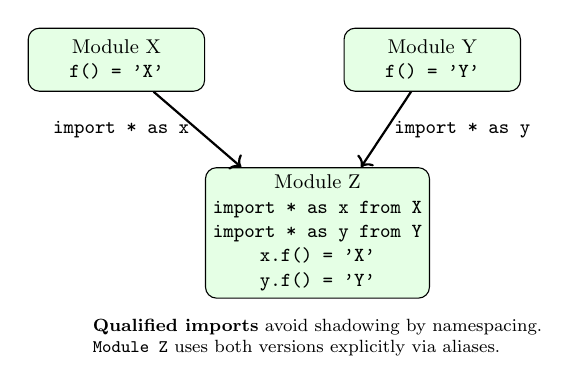
\begin{tikzpicture}[
	scale=0.8, transform shape,
	node distance=1.7cm and 2.2cm,
	every node/.style={font=\small},
	module/.style={rectangle, draw=black, fill=green!10, rounded corners, minimum width=2.8cm, minimum height=1cm, align=center},
	arrow/.style={->, thick}
]

% Modules for Qualified Import Scenario
\node[module] (modX) {Module X\\ \texttt{f() = 'X'}};
\node[module, right=of modX] (modY) {Module Y\\ \texttt{f() = 'Y'}};
\node[module, below right=1.2cm and 0cm of modX] (modZ) {Module Z\\ \texttt{import * as x from X}\\ \texttt{import * as y from Y}\\ \texttt{x.f() = 'X'}\\ \texttt{y.f() = 'Y'}};

% Arrows for Qualified Import Scenario
\draw[arrow] (modX) -- (modZ) node[midway, left] {\texttt{import * as x}};
\draw[arrow] (modY) -- (modZ) node[midway, right] {\texttt{import * as y}};

% Annotation for Qualified Import Scenario
\node[align=left, below=0.2cm of modZ, font=\footnotesize] {
\textbf{Qualified imports} avoid shadowing by namespacing.\\
\texttt{Module Z} uses both versions explicitly via aliases.
};

\end{tikzpicture}

\vspace{1cm} % Add some space between the two diagrams

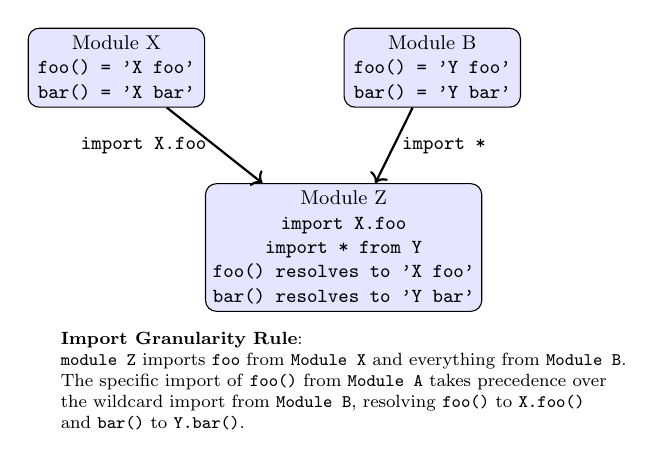
\begin{tikzpicture}[
	scale=0.8, transform shape,
	node distance=1.7cm and 2.2cm,
	every node/.style={font=\small},
	module/.style={rectangle, draw=black, fill=blue!10, rounded corners, minimum width=2.8cm, minimum height=1cm, align=center},
	arrow/.style={->, thick}
]

% Modules for New Scenario (A imports foo, B imports foo & bar)
\node[module] (modX) {Module X\\ \texttt{foo() = 'X foo'}\\ \texttt{bar() = 'X bar'}};
\node[module, right=of modX] (modY) {Module B\\ \texttt{foo() = 'Y foo'}\\ \texttt{bar() = 'Y bar'}};
\node[module, below right=1.2cm and 0cm of modX] (modZ) {Module Z\\ \texttt{import X.foo}\\ \texttt{import * from Y}\\ \texttt{foo() resolves to 'X foo'}\\ \texttt{bar() resolves to 'Y bar'}};

% Arrows for New Scenario
\draw[arrow] (modX) -- (modZ) node[midway, left] {\texttt{import X.foo}};
\draw[arrow] (modY) -- (modZ) node[midway, right] {\texttt{import *}};

% Annotation for New Scenario
\node[align=left, below=0.2cm of modZ, font=\footnotesize] {
\textbf{Import Granularity Rule}:\\
\texttt{module Z} imports \texttt{foo} from \texttt{Module X} and everything from \texttt{Module B}.\\
The specific import of \texttt{foo()} from \texttt{Module A} takes precedence over\\
the wildcard import from \texttt{Module B}, resolving \texttt{foo()} to \texttt{X.foo()}\\
and \texttt{bar()} to \texttt{Y.bar()}.
};

\end{tikzpicture}

\vspace{1cm} % Add some space between the two diagrams

\caption{Module resolution: (a) Conflict resolution with lexical shadowing, where the last import wins. (b) Qualified imports preserve access to all symbols without shadowing by using aliases. (c) Demonstrating the import granularity rule: a specific import of \texttt{foo} from \texttt{moduleA} takes precedence over the general import of everything from \texttt{moduleB}, resolving \texttt{foo()} to \texttt{moduleA.foo()} and \texttt{bar()} to \texttt{moduleB.bar()}.}
\Description{Three module resolution scenarios. In the first two scenarios, module Z inherits from modules X and Y which each define a function f to return a different value. 
Scenario A, conflict resolution with lexical shadowing, where the last import wins: Module Z's import order is X then Y, so module Y's definition shadows modules X's definition and the function resolves to Y's version. 
Scenario B, qualified imports preserve access to all symbols without shadowing by using aliases: Module Z imports all symbols from X and Y but this time gives each of them an alias. The result is that both versions of f can be accessed by using the aliases as namespaces.
In the third scenario, module Z inherits from modules X and Y which each define functions foo and bar to return distinct values.
Scenario C, demonstrating the import granularity rule: a specific import of foo from module X takes precedence over the general import of everything from module Y, resolving foo to X.foo() and bar() to Y.bar().}
\label{fig:module-resolution}
\end{figure}

\subsection{Incremental Inheritance and Differential Reuse}
\label{sec:incremental-inheritance-differential-reuse}

In immutable, content-addressed module systems, every module is identified by a cryptographic hash of its contents. This immutability provides strong guarantees—such as referential transparency, verifiable caching, and decentralized fetch—but it also presents challenges when incremental updates or overrides are needed.

Rather than allowing in-place mutation or overlays, such systems promote \emph{differential reuse} through fine-grained modularization. Reusable logic is factored into small, composable units that can be selectively inherited and extended. When a change is necessary, a new module imports one or more ancestors and extends or overrides their contents, producing a new hash and a new node in the inheritance tree.

These systems are typically language-agnostic, deferring to the host language or runtime to resolve overlapping definitions. Resolution is often governed by a deterministic traversal of the module ancestry graph, such as a topological sort of the Merkle DAG, possibly ordered lexicographically by content hash.

This approach parallels strategies in existing systems: Git commits form immutable DAGs that track content evolution;\footnote{Git's object model ensures immutability and deduplication via SHA-1/SHA-256 content hashes, enabling reproducible version histories.} Nix builds use content-addressed derivations and dependency graphs to isolate and reproduce environments;\footnote{The Nix package manager treats software builds as pure functions, with inputs hashed to ensure deterministic outputs and maximal reuse.} and IPFS organizes files in Merkle DAGs to enable decentralized sharing and incremental updates.\footnote{IPFS (InterPlanetary File System) encodes file versions and directories as Merkle trees, allowing deduplicated and verifiable content exchange.} Promoting fine-grained modularization discourages monolithic library modules in favor of small, single-purpose modules that can be easily transmitted and executed on all manner of host configurations.

Future extensions may explore support for semantic diffs, patch modules, or structured deltas. These approaches could reduce duplication in the module graph, improve resolution performance, and allow for more expressive forms of inheritance without compromising immutability or verifiability.

\section{Optimizations and Caching}
\label{sec:optimizations}

The modular resolution model presented in this paper supports a variety of optimizations that improve both runtime performance and network efficiency, while preserving the determinism and compositionality of the system.

The primary opportunity for optimization lies in the \textit{resolve phase}, during which symbolic references are matched against entries in the reference map and resolved to content-addressed identifiers. Because resolution is deterministic and purely functional with respect to the reference graph, the results of this phase can be cached and reused across executions, contexts, and even deployments.

To support efficient execution, the system defers the fetching and linking of modules until they are actually needed, enabling a form of \textit{lazy loading}. Rather than eagerly loading the full transitive closure of a program's dependencies, the runtime can locate only those modules that are necessary for the execution of a given entry point. This is particularly effective in large module hierarchies or interactive environments, where only a subset of bindings are used in a given session.

The reference graph itself is well-suited to caching, both locally and in networked deployments. Because every node in the graph is identified by a content hash, any resolved module can be safely cached without risk of inconsistency. In distributed settings, resolved modules can be fetched from nearby peers or mirrors, with trust rooted in the immutability of the content hash. This allows for efficient and resilient retrieval of modules without the need for centralized coordination or a trusted registry.

Symbol resolution is further optimized by exploiting structural properties of the reference map. For example, when a symbol is requested, the runtime can avoid unnecessary traversals by using a scoped cache of previously resolved bindings. Because resolution follows a lexically-scoped and shadowing-aware order, these bindings can be reused for subsequent queries in the same context.

Overall, the caching and lazy resolution strategy supports rapid execution, offline availability, and scalable distribution without compromising the reproducibility or auditability of the resulting execution. The modular and immutable nature of the reference graph allows these optimizations to be layered on top of the formal resolution semantics, rather than requiring changes to the resolution model itself.

\subsection{Scalability of Cryptographic Mechanisms}
\label{sec:scalability-crypto}

While Merkle tree-based inheritance offers strong guarantees of immutability, integrity, and reproducibility, it also introduces computational overhead when applied to large module graphs. In large-scale ecosystems, the transitive ancestry of a module may span tens or hundreds of thousands of modules, each contributing to the final Merkle root.

To mitigate this cost, my system implements subtree memoization and batched ancestry hashing. Rather than recomputing the entire tree on every resolution, previously computed subtrees are cached and reused whenever their structure remains unchanged. This significantly reduces both CPU overhead and memory consumption during finalization.

Hash computation is structured as a bottom-up traversal of the module DAG, enabling parallelization across subtrees. This design integrates naturally with distri\-buted build systems and continuous integration pipe\-lines, where isolated subgraphs can be finalized independently and reused across builds.

Importantly, finalized modules are immutable. Their Merkle subtrees can be shared across dependents without duplication, enabling efficient reuse and dramatically reducing redundant hashing. In large registries, this reuse leads to logarithmic rather than linear growth in unique hash entries.

Future extensions may incorporate authenticated data structures, such as vector commitments or sparse Merkle trees, to compress ancestry proofs and further reduce tree depth, particularly for flat or highly reused module hierarchies.

\section{Developer Tooling}
\label{sec:developer-tooling}

A module system grounded in Merkle tree-based inheritance and content-addressed resolution introduces new interaction models for developers. This section outlines the types of tools and developer experiences needed to work effectively with such a system, especially as module graphs grow in size and complexity.

\subsection{Module Graph Visualization}

Inheritance and dependency graphs in Merkle-based systems can grow large and complex, particularly with deep chains of module reuse or broad forks in ancestry. Developer tooling should support interactive graph visualizations, showing both lexical import structure and resolved ancestry. This helps identify where symbols originate, which modules are shadowed, and how resolution paths are computed. Tools should allow filtering by symbol, version, or ancestry to pinpoint specific resolution behaviors.

\subsection{Error Reporting and Diagnostics}

When resolution fails, due to missing modules, unresolved identifiers, or hash mismatches, the system \\should provide rich diagnostics:
\begin{itemize}
	\item Symbol resolution traces showing candidate paths and overrides.
	\item Hash mismatch explanations with expected vs. actual content.
	\item Resolution conflicts with suggestions for disambiguation.
\end{itemize}

Because modules are immutable, ancestry traces are often more informative than runtime stack traces. Tooling should simulate step-by-step resolution paths to clarify precedence and shadowing.

\subsection{IDE and CLI Integration}

Integration with modern IDEs and CLI environments is critical. Features include:

\begin{itemize}
	\item Auto-completion for inherited symbols and re-exports.
	\item Hover-based ancestry and override inspection.
	\item Inline diffs between overridden definitions.
	\item Symbol provenance queries via CLI.
	\item Dry-run simulations of finalization and resolution behavior.
\end{itemize}

Tooling integrates with VS Code, JetBrains IDEs, and common shells, exposing both real-time editing support and CI/CD debugging aids.

\begin{figure}[ht]
\centering
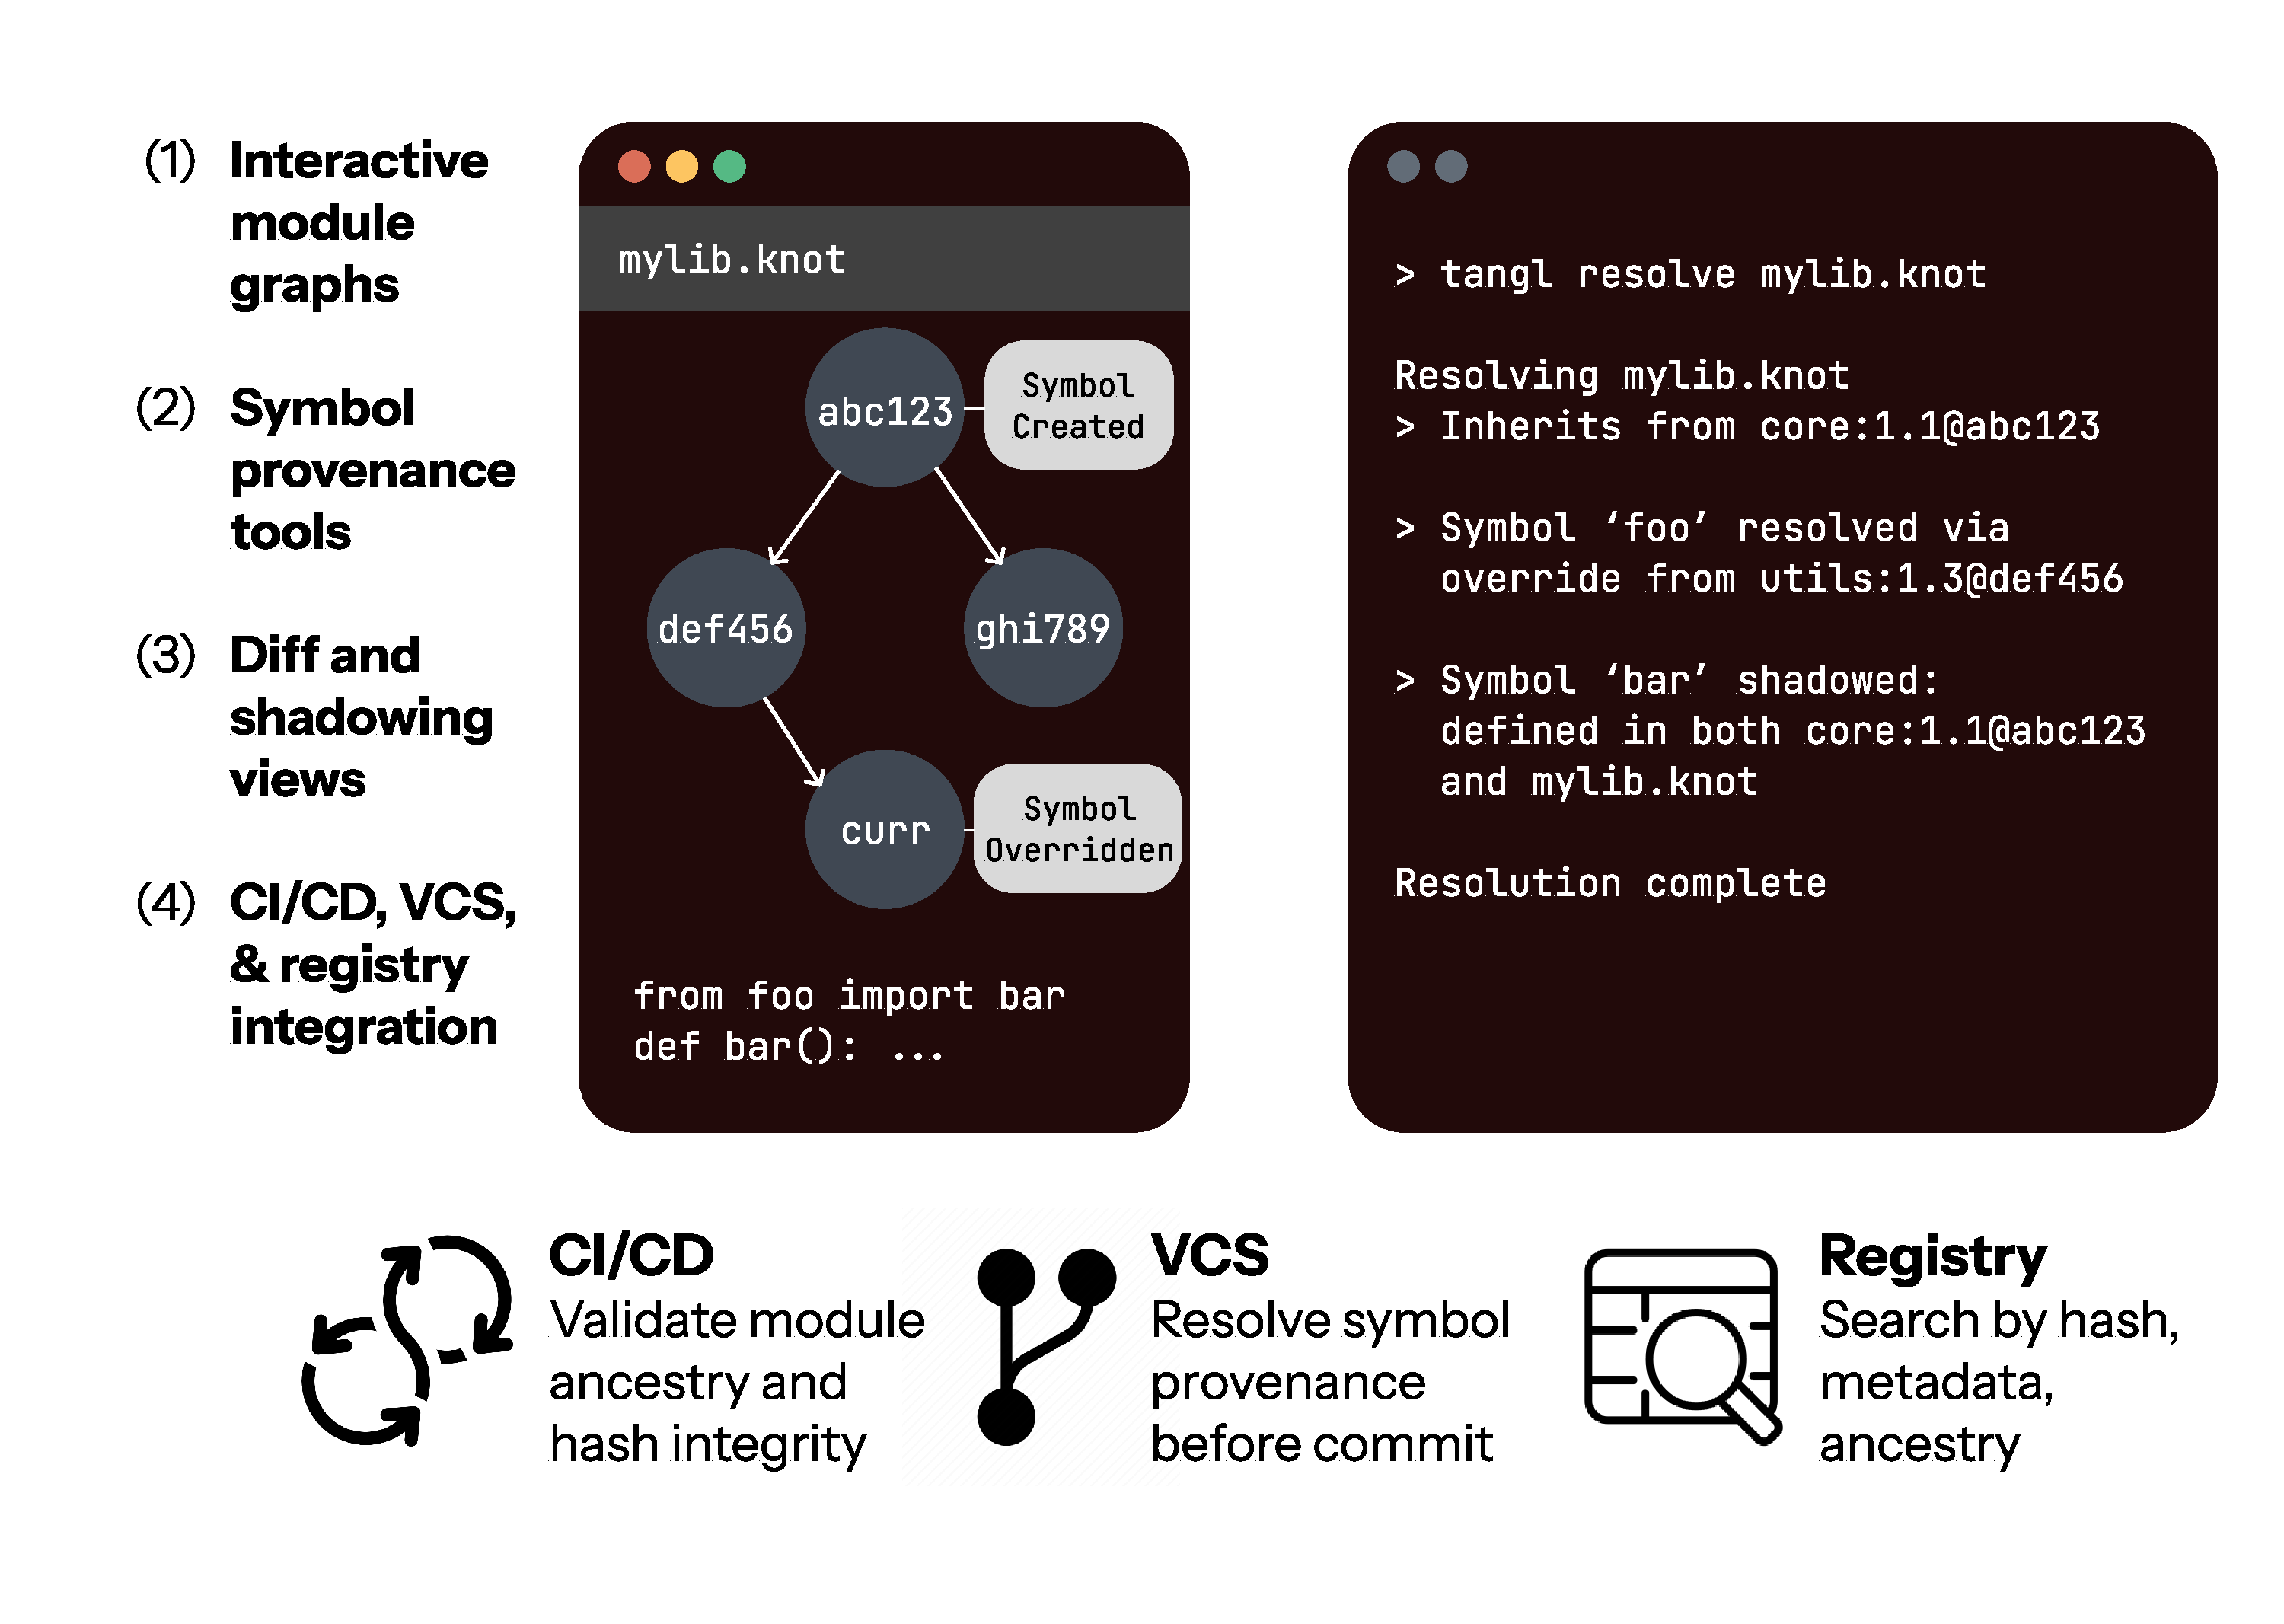
\includegraphics[width=\linewidth]{merkle_inheritance_ux.pdf}
\caption{A conceptual overview of developer tooling for Merkle-based module systems. IDE and CLI tools provide layered insights: (1) interactive module graphs show lexical and resolved ancestry; (2) symbol provenance tools trace resolution across override chains; (3) diff and shadowing views visualize active vs overridden definitions; and (4) integration with CI/CD, VCS, and registries supports reproducibility and ecosystem interoperability.}
\Description{A conceptual overview of developer tooling for Merkle-based module systems. IDE and CLI tools provide layered insights: interactive module graphs in IDEs show lexical and resolved ancestry. Symbol provenance tools trace resolution across override chains. Diff and shadowing views visualize active vs overridden definitions. Integration with CI/CD, VCS, and registries supports reproducibility and ecosystem interoperability.}
\label{fig:tooling}
\end{figure}

\subsection{Debugging Overridden Definitions}

Given the potential for deep inheritance chains and override conflicts, tools should help developers reason about which definitions are active, which are overridden, and why. Especially in the presence of complex MRO-like resolution orders, IDEs or visualization layers should explain precedence and substitution clearly. Symbol diff tools, shadowing inspectors, and override explainers can improve transparency and prevent subtle bugs due to unexpected overrides.

\subsection{Visual Tooling for Symbol Overrides and Ancestry Tracing}
\label{sec:tooling-visuals}

Consider a scenario where a developer hovers over a symbol like \texttt{foo()} in an IDE. The tooling might display:

\begin{itemize}
	\item The Merkle root or alias of the module where \texttt{foo()} was defined,
	\item A linear ancestry of overrides (\texttt{moduleA} $\rightarrow$ \\\texttt{moduleB} $\rightarrow$ \texttt{current}),
	\item Inline diffs for each override.
\end{itemize}

\begin{lstlisting}[language=, caption={Mockup of a symbol override trace as presented in an IDE}, label={lst:override_trace_mockup}, basicstyle=\ttfamily\small]
[Trace] Symbol: foo()
Resolved to:
	moduleC@b17e... (current context)
Override history:
  - moduleC@b17e...
    -> override of foo() [defined inline]
  - moduleB@a9c4...
    -> re-exported from moduleA@d3e1...
  - moduleA@d3e1...
    -> original definition:
function foo() { return 42; }
Ancestry path:
moduleA -> moduleB -> moduleC

- This symbol was overridden in moduleC
[INFO] Click to view diff between 
moduleC::foo and moduleA::foo
\end{lstlisting}

\subsection{Best Practices and Developer Guidance}
\label{sec:best-practices}

To ensure predictable and maintainable behavior, developers should adhere to the following practices:

\paragraph{Avoid Unintentional Shadowing:} Since symbol resolution follows a deterministic merge order, avoid shadowing an imported symbol unless intentionally overriding the logic for that symbol.

\paragraph{Use Explicit Imports for Critical Symbols:} Prefer explicit imports of key symbols when re-exporting from deeply nested modules. \texttt{import(a.foo)} is better than \texttt{import(a)} if you only need to access \texttt{foo}.

\paragraph{Pin Modules Before Finalization:} Always resolve imports to content hashes as soon as you know what functionality you need. This prevents unexpected behavior from the \texttt{latest} tag as new modules are uploaded. 

\paragraph{Document Inheritance Chains:} Document override purposes and expected resolution behaviors. This aids in both auditing and usage of your code.

\paragraph{Validate Resolution with Tooling:} Use diagnostics and linters to confirm that resolution paths are deterministic.

\paragraph{Prefer Compositional Reuse:} Shallow hierarchies simplify debugging and reduce resolution cost. Prefer direct imports over indirect ones, when possible.

\section{Ecosystem Integration and Usability}
\label{sec:ecosystem}

Usability at scale depends not only on local developer tooling but also on system-level integration. This section discusses how Merkle-based modules interact with package managers, CI/CD workflows, and registries.

\subsection{Integration with Existing Package Managers}

The system is designed to interoperate with existing build and package management ecosystems. Compatibility tools can be created to allow developers to continue using \texttt{npm}, \texttt{Cargo}, or \texttt{pip} while gaining immutability and content-based resolution.

\begin{itemize}
	\item \texttt{npm merkle-resolve} would add content hash locking to \texttt{package.json}.
	\item \texttt{cargo finalize} would validate dependency \\graphs before publishing.
	\item \texttt{pip-merk} would overlay Merkle-tracked modules into virtual environments.
	\item etc.
\end{itemize}

These integrations ensure a gradual adoption path for existing codebases.

\subsection{Community and Ecosystem Tooling}

As module systems grow beyond individual projects, ecosystem-facing tools become essential:
\begin{itemize}
	\item Search by hash prefix, semantic version, or ancestry similarity.
	\item Provenance visualization and diffing between \\forks.
	\item Module discovery through public or federated registries.
	\item Moderated publication pipelines for namespaces and groups.
\end{itemize}

Registry APIs expose reproducibility guarantees and ancestry-based filtering, allowing deeper insights into module evolution.

\subsection{UI Affordances and Developer Trust}

Cryptographic guarantees are necessary but not sufficient. Tools should also surface human-readable trust signals:

\begin{itemize}
	\item Verified authorship (e.g., PGP signatures or decentralized IDs).
	\item Maintainer metadata and reputation indicators.
	\item Visualized module forks and merge histories.
	\item Attestations of build reproduction or CI checks.
\end{itemize}

These affordances help developers navigate decentralized module ecosystems with greater confidence.

\subsection{End-User Trust and UI Affordances}
\label{sec:trust-ui}

In decentralized systems where module resolution depends on transitive ancestry, trust becomes not only a cryptographic but also a human-comprehensible property. To make the Merkle-based model approachable for developers, I outline several affordances and UX principles for building trust and transparency into tooling.

\paragraph{Visualizing Ancestry and Inheritance.}
Graphical interfaces should render inheritance hierarchies as DAGs with clear origin points, version labels, and shadowing relationships. By allowing users to inspect a module's full ancestry—down to the hash of each contributing node—tools can make otherwise opaque resolution behaviors auditable and explainable. UI elements such as hover-to-expand ancestry and click-to-trace symbol origin would help users verify correctness and trace override behavior.

\paragraph{Conflict and Shadowing Feedback.}
In cases where symbols are shadowed, redefined, or inherited from conflicting sources, IDEs and CLI tools should surface this information through precise diagnostics. For example, a redefinition should include a warning with the hash and origin of the overshadowed definition, allowing users to distinguish intentional overrides from accidental conflicts.

\paragraph{Provenance and Content Integrity.}
Since all modules are content-addressed, the system guarantees immutability and integrity. To leverage this at the user level, I propose visual markers (e.g., lock icons, color-coded trust levels) indicating whether a module has a known provenance (e.g., signed by a trusted party, linked to a public repository) or is anonymously authored. This also supports audit logs and reproducibility for CI/CD workflows.

\paragraph{Resolution Preview and Explainability.}
Before \\committing to a resolution (e.g., during installation or CI runs), tools should offer a dry-run or preview mode that shows the exact resolved graph, ancestry paths, and expected runtime behavior. This preemptively catches surprises and builds confidence in the decentralized resolution logic.

\paragraph{Fallback and Error Diagnosis.}
If a resolution fails, due to unavailability, conflict, or missing parents, the UI should provide a structured diagnosis: which hash or module could not be fetched, what the fallback path was, and what resolution rule was violated. These diagnostics reinforce the explainability of resolution semantics and empower users to act on failure cases without guessing.

\paragraph{Distributed Trust as a Design Goal.}
Ultimately, the decentralized nature of the system allows users to define their own trust policies: whether to trust modules from known domains, require signatures from specific keys, or enforce reproducible builds. The user interface should expose these policies transparently and allow users to override, escalate, or audit as needed.

\subsection{Trust, Transparency, and Developer Experience}
\label{sec:trust-ux}

To promote transparency and end-user trust in decentralized module systems, I propose several user interface (UI) and user experience (UX) affordances that make module ancestry, versioning, and resolution behaviors visible and auditable.

\paragraph{Human-Readable Provenance.}
Every module \\should expose a navigable ancestry tree derived from its Merkle DAG, displaying inherited modules, shadowed symbols, and override boundaries. This supports debugging and helps developers audit the provenance of imported behavior.

\paragraph{Version Pinning Visualizations.}
In interfaces such as IDEs or web registries, developers should be able to inspect which module versions were finalized, whether exact content hashes or semantic ranges were used, and when hash mismatches are detected due to upstream updates.

\paragraph{Ancestry Conflict Warnings.}
When multiple inherited modules define the same symbol (e.g., via diamond inheritance or multi-parent links), IDEs and command-line tools should emit warnings or previews showing which definition will be resolved, under what rule (e.g., left-to-right linearization), and where ambiguity might arise.

\paragraph{Transparency in Hash-Based Locking.}
To reinforce the integrity guarantees of Merkle-based resolution, tooling should surface which parts of a project are hash-locked, which are open to resolution, and which inherit their lock status from parent modules. This allows users to audit potential supply chain risks at resolution time.

\paragraph{Diff and Override Inspection.}
For any module derived from one or more parents, developers should be able to diff the inherited and modified contents. This capability helps identify whether a derived module introduces functional changes, or simply re-exports behavior from its lineage.

\paragraph{Registry and Peer Provenance.}
In decentralized contexts, trust also depends on the source of modules. Tools should display metadata about which registry or peer contributed each resolved module, along with verification of its hash and ancestry. This reduces trust assumptions and helps detect impersonation or mispublishing.

These affordances are critical for developer confidence in decentralized and inheritance-based systems. While the underlying resolution machinery is content-addressed and formally sound, user interfaces must make this machinery explainable and traceable for real-world adoption.

\begin{figure}[ht]
\centering
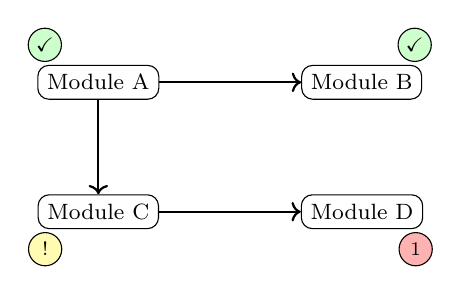
\begin{tikzpicture}[
	module/.style={rectangle, draw=black, rounded corners, minimum height=1.2em, minimum width=3em, align=center, font=\footnotesize},
	trust/.style={circle, draw=black, fill=green!20, inner sep=1pt, font=\scriptsize, minimum width=1.2em},
	warn/.style={circle, draw=black, fill=yellow!30, inner sep=1pt, font=\scriptsize, minimum width=1.2em},
	danger/.style={circle, draw=black, fill=red!30, inner sep=1pt, font=\scriptsize, minimum width=1.2em},
	edge/.style={->, thick},
]

% Nodes
\node[module] (A) {Module A};
\node[module, right=1.8cm of A] (B) {Module B};
\node[module, below=1.2cm of A] (C) {Module C};
\node[module, right=1.8cm of C] (D) {Module D};

% Trust indicators
\node[trust, above left=0.1cm and -0.25cm of A] (TA) {\checkmark};
\node[trust, above right=0.1cm and -0.25cm of B] (TB) {\checkmark};
\node[warn, below left=0.1cm and -0.25cm of C] (TC) {!};
\node[danger, below right=0.1cm and -0.25cm of D] (TD) {{\fontencoding{U}\fontfamily{futs}\selectfont\char 49\relax}};

% Edges
\draw[edge] (A) -- (B);
\draw[edge] (A) -- (C);
\draw[edge] (C) -- (D);

\end{tikzpicture}
\caption{A trust overlay on the module graph. Each node represents a module, annotated with a trust indicator: green check for verified maintainers, yellow exclamation for unsigned modules, and red warning for known issues or missing signatures. This overlay aids users in evaluating dependency trustworthiness.}
\Description{A trust overlay on the module graph. Each node represents a module, annotated with a trust indicator: green check for verified maintainers, yellow exclamation for unsigned modules, and red warning for known issues or missing signatures. This overlay aids users in evaluating dependency trustworthiness. The diagram shows 4 modules}
\label{fig:trust-overlay}
\end{figure}

\subsection{Ecosystem Compatibility and Developer Trust}

Maintaining compatibility with existing systems also helps build trust. Developers are more likely to adopt new infrastructure if it complements their existing tooling and requires minimal disruption. This includes supporting familiar metadata formats, dependency declarations, and tooling conventions. Moreover, reproducibility guarantees provided by content-addressed modules can enhance security and build integrity in existing workflows.

\section{Integration with Existing Ecosystems}
\label{sec:integation-existing-ecosystems}

While content-addressed, Merkle-based module systems offer significant advantages in immutability, caching, and reproducibility, integration with existing language and package ecosystems remains a key challenge. Developers rarely adopt systems in isolation; instead, they require interoperability with current tools, workflows, and dependency managers.

\subsection{Migration Strategies and Tooling for Legacy Codebases}
\label{sec:migration-strategies}

To support gradual migration from semver-based systems, my approach uses bridge layers that interpret legacy version constraints (e.g., \verb#"foo": "^1.3.0"#) and resolve them to concrete versions using the host ecosystem's native resolver (e.g., \texttt{npm}, \texttt{Cargo}). The resulting version (e.g., \texttt{1.3.5}) is then compared against the registry to map it to a finalized Merkle root.

If the registry contains a matching resolution, the import is replaced with the corresponding content hash. If no match is found, the system can fall back to the traditional package manager to fetch and hash the package. This preserves deterministic resolution while allowing continued use of familiar semver workflows.

These bridges operate strictly at the local level: legacy semver-based imports are resolved to Merkle identifiers prior to module finalization and are not stored or propagated in the DHT. This ensures that all modules published to the distributed registry use content-based addressing exclusively, maintaining consistency and determinism across the network.

The registry serves as a shared, verifiable cache of resolved legacy imports, enabling consistent and reproducible results across environments. As more packages are pinned and published in content-addressed form, projects can progressively move away from semver-based workflows without sacrificing compatibility. Because semver metadata can be optionally attached to newly finalized modules, developers may continue to use semver constraints locally—even after dependencies have been fully resolved and published. This remains viable as long as bridge layers attempt resolution through the registry first, falling back to the host package manager only when necessary.

Migration tooling can support this process with: 
\begin{itemize} 
	\item \textbf{Bridge-assisted diffing}: Detecting changes between local graphs and published Merkle mappings. 
	\item \textbf{Semantic hashing}: Converting legacy packages into content-addressed modules with symbol-pre\-serving boundaries. 
	\item \textbf{Dry-run simulations}: Previewing how semver imports will resolve under Merkle semantics. 
\end{itemize}

This strategy supports incremental adoption without disrupting existing toolchains, while gradually shifting dependency resolution to a globally verifiable, content-addressed model.

\subsection{Incremental Migration Patterns}
\label{sec:incremental-migration}

Migration to a content-addressed module system can proceed incrementally, without disrupting existing \\workflows. Adoption typically begins at leaf nodes in the dependency graph, internal libraries, stable third-party modules, or standalone utilities, which can be finalized and published independently. These modules are wrapped in Merkle-resolved snapshots and registered for reuse without requiring upstream coordination.

Consumers of finalized modules can then migrate by replacing semver imports with Merkle references. This transition requires no source changes to dependent modules and progressively improves reproducibility. Hybrid states, where some modules use semver and others use content hashes, are fully supported by the registry semantics (Section~\ref{sec:namespace-based-registry}), enabling gradual migration across teams or repositories.

Tooling can assist by identifying unresolved dependencies, flagging mutable imports, and suggesting \\content-addressed upgrades. Over time, these practices yield fully Merkle-resolved graphs with deterministic builds and traceable ancestry, without invasive code rewrites.

\subsection{Interoperability and Compatibility with Existing Ecosystems}
\label{sec:interoperability-existing}

My model supports seamless integration with existing package managers (e.g., \texttt{npm}, \texttt{Cargo}, \texttt{pip}) by translating semver constraints into content-addressed identifiers. For example, a dependency like \texttt{rand = "0.8"} is resolved against registry metadata to a specific Merkle root (e.g., \texttt{rand@0.8.5 → QmZ9...abc}), which is then used for all resolution and validation.

\paragraph{Integration Highlights}
\begin{itemize}
	\item \textbf{Performance:} Semver resolution incurs \\overhead, but each version is uniquely content-addressed, eliminating ambiguity.
	\item \textbf{Compatibility:} Lockfiles are replaced by immut\-able bindings but can be layered atop existing tooling.
	\item \textbf{Usability:} Tools display semver metadata alongside hashes and offer workflows to map between them.
\end{itemize}

\paragraph{Design Challenges}
\begin{itemize}
	\item \textbf{Semver Divergence:} Varying semver semantics across ecosystems complicate unified resolution.
	\item \textbf{Multiple Versions:} Each version resolves to a distinct Merkle root, making duplications explicit and manageable.
\end{itemize}

\paragraph{Bridging Strategies}
\begin{itemize}
	\item \textbf{Pinning:} Semver ranges are resolved and pinned to Merkle hashes, enabling reproducibility and reverse lookup.
	\item \textbf{Annotated Metadata:} Merkle roots retain semver annotations for transparency.
	\item \textbf{Layered Resolution:} Local lockfiles and registry-based resolution can coexist, supporting hybrid workflows.
\end{itemize}

These mechanisms ensure a smooth migration path without compromising determinism or compatibility.

\section{Interoperability and Protocols for Real-World Systems}
\label{sec:interoperability-real-world}

Interoperability with existing package management systems such as \texttt{npm}, \texttt{Cargo}, and \texttt{Solidity} is central to the adoption of the proposed decentralized module registry. However, challenges arise when reconciling versioning schemes, particularly with respect to transitive dependencies and version mismatches between systems.

\subsection{Handling Transitive Dependencies}
One of the core challenges in integrating a decentralized system with traditional package managers is resolving transitive dependencies. In conventional systems like \texttt{npm}, dependencies often specify ranges of versions, leading to the possibility of version inflation and conflicts when dependencies overlap across packages. In contrast, my system uses deterministic Merkle hashes to resolve each dependency to a specific module version. This eliminates ambiguity but raises the need for a robust conflict resolution mechanism when transitive dependencies across systems result in mismatches.

I propose the following strategies for resolving version conflicts:

\begin{itemize}
	\item \textbf{Priority Ordering:} When conflicts occur, the system can prioritize higher-level dependencies to avoid circular dependency resolution or duplication. Dependencies with stricter version requirements take precedence over looser ranges.
	\item \textbf{Range-to-Hash Mapping:} I propose a flexible mapping between semver version ranges and Mer\-kle hashes. The system can automatically \\translate version ranges into the closest matching content-addressed version, allowing cross-system compatibility.
	\item \textbf{Conflict Resolution API:} An API will provide developers with insights into why conflicts occur and offer suggestions for resolving them. This can include proposing alternative versions, merging ranges, or creating forked dependencies.
\end{itemize}

\subsection{Version Mismatch Handling}
\label{sec:version-mismatch}

While my system ensures deterministic resolution thr\-ough Merkle-based identifiers, integration with ecosystems that rely on semantic versioning introduces potential mismatches in expectations. Traditional systems like \texttt{npm} may resolve a version range to different concrete versions over time, whereas Merkle roots represent fixed, immutable snapshots. When bridging these systems, the challenge is not just resolution but communicating intent and compatibility clearly.

To support hybrid workflows and reduce developer confusion, I introduce the following mechanisms:

\begin{itemize}
	\item \textbf{Version Bridge Adapters:} Adapters translate semver constraints into Merkle roots at resolution time and preserve this mapping in metadata. These bridges allow existing semver declarations to function as expected, while ensuring that once resolved, all dependencies are pinned immutably for reproducibility.
	\item \textbf{Compatibility Hints and Warnings:} To surface mismatches early, the system can analyze metadata and structural differences between modules resolved from semver constraints. For example, if two modules claim semver compatibility but differ significantly in their Merkle lineage, tools may flag the resolution as potentially unsafe or inconsistent with semver expectations.
\end{itemize}

These features are designed to make interoperability safer and more transparent, especially during the transition from traditional versioning to fully content-addressed module resolution.

\subsection{Security Implications}

With a decentralized system, the integrity and security of the module graph depend on the trustworthiness of the content hashes and the associated module metadata. However, integrating with external systems introduces the risk of malicious updates or erroneous versioning. To address these concerns, I rely on cryptographic signatures to authenticate module sources, ensuring that only authorized publishers can publish updates. Additionally, the system can integrate with existing security protocols (e.g., \texttt{npm}'s audit feature) to provide developers with security alerts about potential vulnerabilities in third-party modules.

\section{Scalability in Large Distributed Registries}
\label{sec:scalability-distributed}

In globally distributed settings with millions of modules, scalability becomes critical. The proposed system uses a content-addressed DHT (Distributed Hash Table) for resolution, where each node can cache subtrees of the Merkle module graph. To evaluate scalability, future work should measure metrics such as:
\begin{itemize}
	\item \textbf{Average DHT hop count} for resolution queries under varying node churn rates.
	\item \textbf{Cache hit rates} across popular modules, considering both first-party imports and indirect ancestry.
	\item \textbf{Resolution throughput} under simulated load across geographically distributed peers.
\end{itemize}

To mitigate unreliable networks or partial availability, each module's ancestry path can be requested independently in parallel, with redundancy strategies (e.g., Kademlia's $k$-bucket querying or erasure coding) used to increase resilience. Caching policies based on usage patterns and predictive prefetching could also reduce remote lookups.

I also plan to explore hierarchical DHT overlays and regional replication zones, allowing popular modules to propagate more aggressively in high-traffic regions. These directions will guide both practical deployment and formal scalability modeling.

Theoretically, the system's architecture benefits from logarithmic lookup time due to the DHT's structure. Because modules are content-addressed and immutable, resolution can proceed by independently fetching and caching Merkle subtrees. This allows decentralized, parallel resolution across nodes and minimizes redundant fetches even as the registry scales to millions of modules.

\section{Security Considerations}

The use of cryptographic hashes and Merkle trees in this system ensures that modules and their ancestry are tamper-resistant. However, there are potential attack vectors to consider:

\paragraph{Hash Collision Attacks:} While cryptographic hash functions such as SHA-256 are widely considered secure, hash collisions could theoretically lead to multiple different modules having the same identifier. To mitigate this risk, I recommend using SHA-256 or higher, which offers a large enough output space to make collisions highly improbable. Additionally, I use Merkle trees to provide a unique fingerprint of module ancestry, making it extremely difficult to alter a module's content without detection. Finally, both the registry and the module store enforce immutability: once a module or registry entry is created, it cannot be overridden or edited. As a result, any attempt to insert a hash-colliding module would fail, preserving integrity and preventing ambiguous resolutions.


\paragraph{Sybil Attacks in the Registry:} To ensure the integrity of the distributed registry, I employ public key cryptography to sign namespace Merkle roots, ensuring that only the owner of a namespace can modify its entries. Clients must verify these signatures before accepting updates, protecting against unauthorized modifications.

\paragraph{Replay Attacks:} To prevent replay attacks, where an attacker might reuse a previously finalized module in an unintended context, each finalization event includes a cryptographically signed timestamp and context-specific metadata. This binding ensures that a module finalized for one purpose or environment cannot be silently replayed in another without detection. Any mismatch in context or timestamp would invalidate the signature, making unauthorized reuse evident and verifiable.

\paragraph{DoS Resilience:} Content-addressed module systems can mitigate denial-of-service (DoS) attacks, such as hash bomb or modules with excessive fan-out, by enforcing configurable limits on resolution depth and import breadth. These thresholds can be set based on empirical norms observed across healthy module graphs, such as median fan-out per module or typical dependency tree depth in a given ecosystem. Modules exceeding these bounds may be rejected or require explicit overrides. Lazy resolution strategies further enhance resilience by fetching only the required subtrees of the dependency graph, limiting exposure to malformed or excessive structures.

\subsection{Expanded Security Threat Model}

In addition to the attack methods already discussed, I also consider network partitioning and module unavailability as potential security risks. To mitigate partitioning, the system utilizes a decentralized module resolution approach, which allows nodes to resolve modules independently, even when parts of the network are unavailable.

Moreover, the system's caching mechanism is designed to prevent exploitation. If a malicious actor attempts to cache incorrect or outdated modules, the system checks the integrity of cached modules using cryptographic proofs before allowing their use.

I also address potential exploits related to module unavailability. If a module is unavailable due to network failure or malicious interference, the system gracefully falls back to local caches, and the developer is notified with an appropriate error message, ensuring minimal disruption.

\subsection{Future-Proofing Hash Function Security}
\label{sec:security-future}

While SHA-256 currently provides strong preimage and collision resistance, long-term security requires anticipating future cryptographic threats, including those posed by quantum computing. Post-quantum cryptographic research has produced several candidate hash functions, such as those based on the SPHINCS+ and XMSS families, which offer resistance to quantum attacks at the cost of larger output sizes and slower performance.

Future work includes evaluating these alternative hashing algorithms for suitability in content-addressed module systems, focusing on compatibility with Merkle tree constructions, registry performance, and adoption viability. Additionally, migration strategies may be developed to support gradual transition between hash functions, including hybrid hash encoding schemes or dual-hash identifiers that preserve backward compatibility while enabling forward security. By future-proofing the core cryptographic primitives of the system, I aim to maintain integrity guarantees even in the face of emerging threats.

\section{CI/CD and VCS Integration (Supplementary)}
\label{sec:ci-vcs-integration}

A detailed discussion of how the proposed system integrates with continuous integration (CI) workflows and version control systems (VCS), including semantic conflict detection, immutable tagging, and cache-aware builds, is included in the supplementary materials (Appendix~\ref{supp-appendix:ci-vcs}).

\begin{table*}[t]
\centering
\caption{Synthetic Benchmark Summary}
\label{tab:synthetic-benchmarks}
\begin{tabular}{@{}lll@{}}
\toprule
\textbf{Benchmark}           & \textbf{Setup}                         & \textbf{Result}                   \\ \midrule
Finalization Time            & Linear chains (depth \(N\))            & Linear scaling in \(N\)           \\
Symbol Lookup Latency        & Repeated lookups in cached graphs      & Sublinear (amortized) due to caching \\
Graph Compression            & Diamond graphs with shared ancestors   & 60–80\% subtree reuse             \\ \bottomrule
\end{tabular}
\end{table*}

\section{Evaluation and Testing Methodology}
\label{sec:evaluation}

I outline the evaluation goals and empirical validation plan for my Merkle-based module system. While a full implementation is still in development, I report preliminary findings based on synthetic data and provide a roadmap for testing real-world performance, scalability, and usability. Complete benchmark configurations, generated results, and synthetic graph structures are provided in the supplementary materials.

\subsection{Evaluation Goals}

My evaluation strategy targets the following questions:

\begin{itemize}
	\item How does resolution performance scale with \\graph width, depth, and ancestry reuse?
	\item How robust is the system under partial failures or adversarial input?
	\item Can inheritance semantics preserve determinism and modularity in practice?
\end{itemize}

These goals inform the benchmarks and testing workflows I prioritize.

\subsection{Prototype Development}

I will implement a reference prototype in \texttt{Rust}~\cite{rust} using \texttt{libp2p}~\cite{libp2p} for decentralized communication and \texttt{Wasmer}~\cite{wasmer} for WebAssembly execution. This prototype will serve as the basis for full-scale empirical validation.

\subsection{Future Testing Plan}

Empirical testing will evaluate:

\begin{itemize}
	\item Latency and memory usage across large dependency graphs.
	\item Resolution correctness under stale caches and node dropout.
	\item Conflict handling in symbol shadowing and multi-parent inheritance.
	\item Developer-facing tooling for visualization, debugging, and traceability.
\end{itemize}

Testing will simulate real-world workflows (e.g., \\CI/CD, interactive development) to assess usability and performance.

\subsection{Supplementary Benchmarks and Testing Scenarios}
\label{sec:supplementary-benchmarks}

Detailed benchmark results from synthetic module \\graphs, as well as comparative analyses with existing tools (e.g., \texttt{npm}, \texttt{Cargo}, \texttt{pip}), are available in the supplementary materials. These include:

\begin{itemize}
	\item Synthetic benchmarks on finalization, symbol resolution, and structural compression.
	\item Stress tests for network partitioning, stale ancestry, and fallback performance.
	\item Metrics such as average DHT hops, cache hit rates, and deduplication efficiency.
	\item Simulated workflows including dependency graph rebuilding and distributed editing.
\end{itemize}

These results offer preliminary insights into the system's expected behavior and scalability.

\paragraph{Supplementary Materials.}
Due to space constraints, full details of my synthetic benchmark methodology, prototype development plan, and empirical evaluation scenarios are provided in the supplementary materials. These include synthetic results, proposed metrics, testing workflows, and comparative analysis with existing systems.

\section{Limitations and Future Work}
\label{sec:limitations-future}

Although the Merkle tree-based inheritance model provides strong guarantees of determinism, integrity, and compositionality, several limitations remain:

\begin{itemize}
	\item \textbf{Performance on modules with many direct parents.} 
	Finalization hashes the set of direct parent IDs. A large number of parents—now including atomic groups—can increase sorting and hashing overhead.
	\item \textbf{Recursive groups complexity.} 
	SCC detection and group serialization introduce additional build-time work. Extremely large recursive groups may challenge memory and canonical ordering.
	\item \textbf{Registry dependency.} 
	Symbolic imports rely on a distributed registry. Network failures or malicious updates can block resolution unless clients maintain robust caches and fallback strategies.
	\item \textbf{Limited language-specific typing.} 
	We rely on side-car metadata for exported symbol types. Full support for parametric polymorphism, type class\-es, and richer type-level constraints remains to be integrated.
	\item \textbf{Tooling maturity.} 
	IDE plugins, visual diff tools, and override inspectors exist only as prototypes. Production-ready developer experiences are essential for adoption.
\end{itemize}

\subsection{Future Work}

To address these limitations and broaden the model's applicability, I plan to explore:

\begin{itemize}
	\item \textbf{Authenticated data-structure optimizations.}
	Leverage sparse Merkle trees or vector commitments to compress large parent sets and support constant-size proofs.
	\item \textbf{Graph deltas and patch modules.}
	Introduce differential inheritance modules that encode only changes relative to a parent, reducing duplication and speeding up finalization.
	\item \textbf{Richer type systems.}
	Formalize and mechanize generic type aliases, subtype constraints, and \\module-level interface contracts within the finalization framework.
	\item \textbf{Zero-knowledge proofs of lineage.} 
	Enable \\privacy-preserving verification by proving ancestry inclusion without revealing module contents.
	\item \textbf{Robust registry protocols.} 
	Design decentralized consensus or reputation schemes to guard against Sybil attacks, equivocation, and unauthorized updates.
	\item \textbf{Compilers and linkers as modules.} 
	Model compiler frontends, optimizers, and linkers as Merkle-rooted modules, enabling fully decentralized, reproducible build pipelines in which each compilation stage is content-addressed and verifiable.
	\item \textbf{Ecosystem integration.} 
	Develop production-\\grade adapters for npm, Cargo, pip, CI/CD systems, and IDEs to support incremental migration and seamless workflows.
\end{itemize}

\section{Conclusion}
\label{sec:conclusion}

I have presented a Merkle tree-based inheritance model that treats each module as a cryptographic commitment to both its code and its resolved dependencies. By hashing only the finalized parent IDs, each of which already embeds its full ancestry, finalization remains efficient, deterministic, and tamper-proof. Symbol resolution follows a fixed, breadth-first merge order, producing unambiguous override traces and enabling fine-grained module composition without mutable registries or lockfiles.

My prototype implementation, Tangl, demonstrates how these ideas can integrate with existing ecosystems via semver translation adapters and decentralized registries. I have also stated the core metatheoretic properties of determinism, injectivity, and compositionality in the main text.

For complete pseudocode of the finalization algorithm, mechanized proofs of the lean theorems, and a formal mapping to existing module calculi, please consult the supplementary materials.

\balance


\bibliographystyle{ACM-Reference-Format}
\bibliography{bibliography}

\end{document}
